\chapter{\label{ch:2-gb-method}A method to find ghost populations using genome-wide genealogies}

\minitoc

\section{Chapter overview}
In this chapter, we introduce GhostBuster, a novel method designed to identify admixture events by analyzing genome-wide genealogies inferred from genomic variation data. GhostBuster functions as a mixture model, probabilistically clustering local trees into distinct groups using an efficient expectation-maximization algorithm. The method can be understood as an iterative process consisting of two key steps. First, given multiple potential coalescence rates with a set of reference populations, GhostBuster assigns each genomic region of the target individual to one of these coalescence rates (see Figure \ref{fig:gb-simplified-overview}A). In the second step, it refines these coalescence rate estimates by utilizing the local ancestry information derived from the first step, similar to estimating cluster means and covariances in Gaussian mixture models (see Figure \ref{fig:gb-simplified-overview}B). The coalescence rates and proportions are randomly initialized.

We begin by presenting the theoretical framework underlying GhostBuster in Section \ref{sec:ch2-gb-theory}, where we employ coalescent theory to model the observed genealogies. Next, in Section \ref{sec:ch2-gb-method}, we delve into the algorithmic and methodological details of the method. In Section \ref{sec:ch2-gb-data} we discuss the various modern and ancient DNA resources we use in the analyses and how we construct genealogies. In section \ref{sec:ch2-gb-sim}, we apply GhostBuster to two simulated scenarios to demonstrate its ability to recover ghost admixture events, performing several ablation studies to explore different aspects of the method. Finally, in Section \ref{sec:ch2-gb-real}, we apply GhostBuster to real data, identifying some previously known admixture signals and comparing the local ancestry estimates with previous estimates to showcase the method's robustness.

% a figure showing the iteration between inferring coal. rates and inferring local ancestry

\begin{figure}[h!]
    \centering
    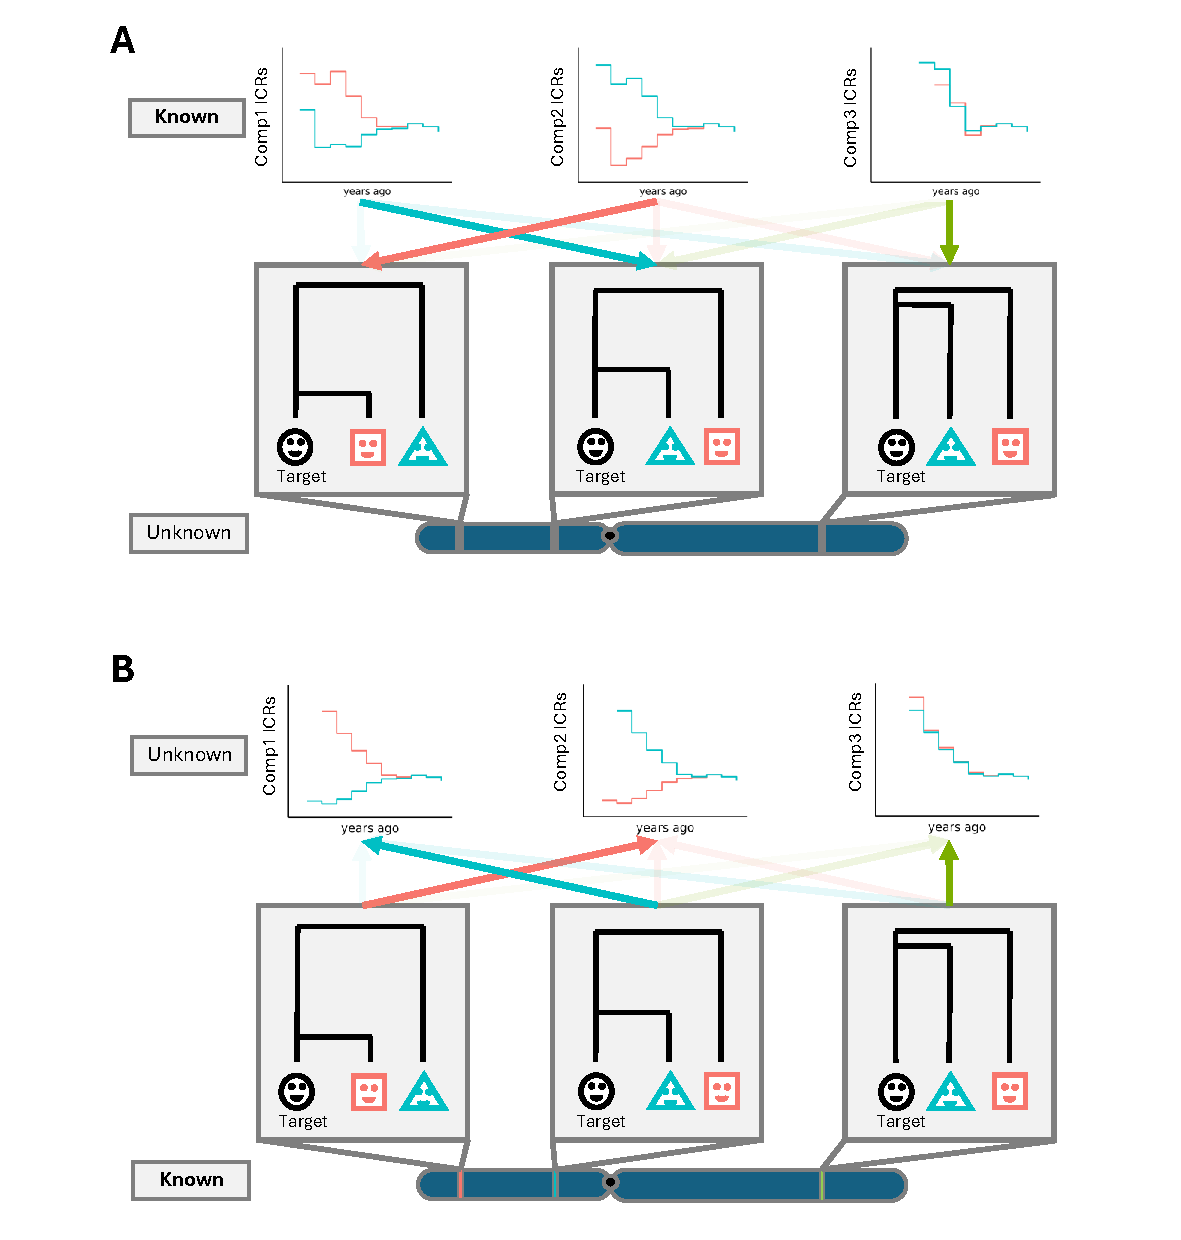
\includegraphics[width=\textwidth]{figures/thesis_gb_simplified_overview.pdf}
    \caption{\textbf{A simplified overview of GhostBuster.} GhostBuster implements an iterative expectation-maximization (EM) algorithm which cycles between two states A and B. (A) inferring local ancestry of a target individual given multiple coalescence rates of the target individuals with a set of reference populations. (B) using the local ancestry to refine the estimates of coalescence rates of target individual and the reference populations.}
    \label{fig:gb-simplified-overview}
\end{figure}

\section{Theoretical framework for our method}
\label{sec:ch2-gb-theory}

\subsection{Introduction to mixture models}

Mixture models are a general class of probabilistic models used to represent the presence of subpopulations within an overall population, even when there is no explicit identification of subpopulation membership for individual observations. Essentially, they assume that the data being analyzed is generated from a mixture of several different distributions, where each distribution corresponds to a different subpopulation or cluster. 

\subsubsection{Gaussian mixture models}

One of the simplest and most widely used mixture models is the Gaussian Mixture Model (GMM). Let's assume the data is sampled from a mixture of two Gaussian distributions with different means. The GMM assumes that each data point $\mathbf{x}$ is generated from one of these Gaussian distributions. Mathematically, the model is expressed as:
\begin{equation}
p(\mathbf{x}) = \pi_1 \mathcal{N}(\mathbf{x} \mid \mu_1, \Sigma_1) + \pi_2 \mathcal{N}(\mathbf{x} \mid \mu_2, \Sigma_2)
\end{equation}

where, $\pi_1$ and $\pi_2$ are the proportions of being in either one of the clusters, satisfying $\pi_1 + \pi_2 = 1$, and $(\mu_1, \Sigma_1)$ and $(\mu_2, \Sigma_2)$ are the parameters of the two Gaussians. Therefore the parameters to be inferred from the observed samples are $(\pi_1, \mu_1, \Sigma_1, \mu_2, \Sigma_2)$. The inference of the parameters is often carried out using the expectation-maximization (EM) algorithm \cite{dempster1977maximum}.

The EM algorithm operates by probabilistically inferring hidden variables under the model in the E-step, and using these hidden variables to simplify and analytically maximize the likelihood in the M-step. In the Gaussian Mixture Model, the hidden variables are the cluster memberships of each data point. The EM updates for Gaussian Mixture Models proceed as follows:

\begin{enumerate}
    \item E-step: Compute the expected log-likelihood of the data conditioned on the current estimates of the parameters. For Gaussian Mixture Models, this involves calculating the posterior probabilities that a data point belongs to a Gaussian distribution:
    \begin{equation}
        \gamma_{i}(\mathbf{x}_j) = \frac{\pi_i \mathcal{N}(\mathbf{x}_j \mid \mu_i, \Sigma_i)}{\sum_{k=1}^{2} \pi_k \mathcal{N}(\mathbf{x}_j \mid \mu_k, \Sigma_k)}
    \end{equation}
    where, $\gamma_{i}(\mathbf{x}_j)$ is the hidden variable that represents the probability that the data point $\mathbf{x}_j$ was generated by the $i$-th Gaussian distribution. 
    \item M-step: Uses the hidden variable to maximize the expected log-likelihood and estimate updated parameters:
    \begin{align}
        \pi_i^{\text{new}} &= \frac{1}{N} \sum_{j=1}^{N} \gamma_{i}(\mathbf{x}_j)  \nonumber \\
        \mu_i^{\text{new}} &= \frac{\sum_{j=1}^{N} \gamma_{i}(\mathbf{x}_j) \mathbf{x}_j}{\sum_{j=1}^{N} \gamma_{i}(\mathbf{x}_j)} \nonumber \\
        \Sigma_i^{\text{new}} &= \frac{\sum_{j=1}^{N} \gamma_{i}(\mathbf{x}_j) (\mathbf{x}_j - \mu_i^{\text{new}})(\mathbf{x}_j - \mu_i^{\text{new}})^\top}{\sum_{j=1}^{N} \gamma_{i}(\mathbf{x}_j)}
    \end{align}
\end{enumerate}

It can be shown that iterating between the E- and M-steps leads to non-decreasing log-likelihood updates. An illustration of the model fitting for a 2-dimensional mixture of Gaussians is shown in Figure \ref{fig:gb-gmm-visualize}.

\begin{figure}
    \centering
    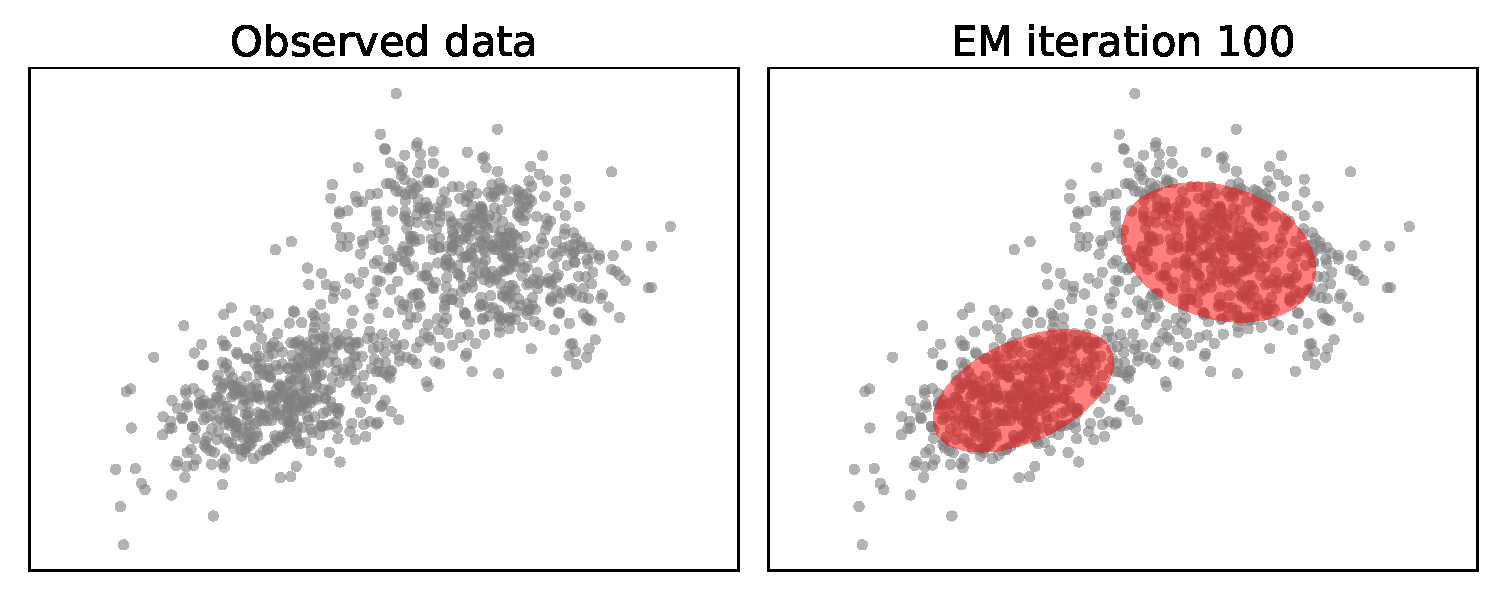
\includegraphics[width=\textwidth]{figures/gmm_visualize.pdf}
    \caption{\textbf{Gaussian mixture model.} The observed data and inferred clusters using the Gaussian mixture model after 100 EM iterations, the Gaussian mixtures inferred are represented by the red ellipse.}
    \label{fig:gb-gmm-visualize}
\end{figure}

\subsection{Mixture model for the coalescent}
\label{the_model}
We aim to extend the basic example of mixture models to genealogies by specifically modeling coalescence events on a given target lineage as a mixture distribution. The input for our method consists of at each site which individuals and at what times (or reference populations) the target sample coalesces as we move backward in time. Our goal is to model this as a mixture distribution, clustering locations based on `differences' in the coalescence histories of the target lineage. The expected output of our model is a per-component coalescence rate matrix, which defines how the target individual coalesces with a set of reference population within each specific component of the mixture.

Our method capitalizes on the fact that admixtures can be characterized by these coalescence rates with a set of reference populations. To illustrate this, consider the example of Denisovan admixture in Papuans. It is well known that Papuans carry up to 5\% Denisovan ancestry in their genomes. This archaic ancestry is distinct from the majority of Papuan ancestry, as the regions with Denisovan admixture exhibit more frequent coalescence events with Denisovans but do not coalesce with modern human lineages until the time of the Denisovan-human split. Therefore, there is a clear difference in the coalescence history between archaic and non-archaic genomic regions in Papuans, which we leverage to infer admixture.

We use the coalescent framework to model coalescence times along a lineage as an exponential distribution, where coalescence rates are determined by the population distribution of the clade coalescing with the target lineage. We have already derived a closed-form solution for the Maximum Likelihood Estimate (MLE) of coalescence rates for a pair of lineages (see Section \ref{sec:ch1-gb-theory}). This maximum likelihood estimate can be extended to multiple samples by treating each pair of lineages independently and multiplying the likelihood across all pairs. This approach is used to estimate effective population sizes and cross-population coalescence rates in PSMC \cite{li2011inference}, a widely used tool for inferring population history from genetic data. 

Although the pairwise likelihood approach is straightforward, it assumes that each pair of lineages is independent, even though they are highly structured and interdependent. To address this limitation, we extend the likelihood of observing coalescence events by conditioning on the inferred tree topology at each genomic site. More formally, we model the probability of a target lineage coalescing with any remaining lineage using a non-homogeneous Poisson process. To simplify the model, we assume that the coalescence rate of a lineage is proportional to the weighted sum of the coalescence rates of its descendants, as inferred from the tree at that site (see Figure \ref{fig1} for an example).

\begin{figure}[h!]
    \centering
    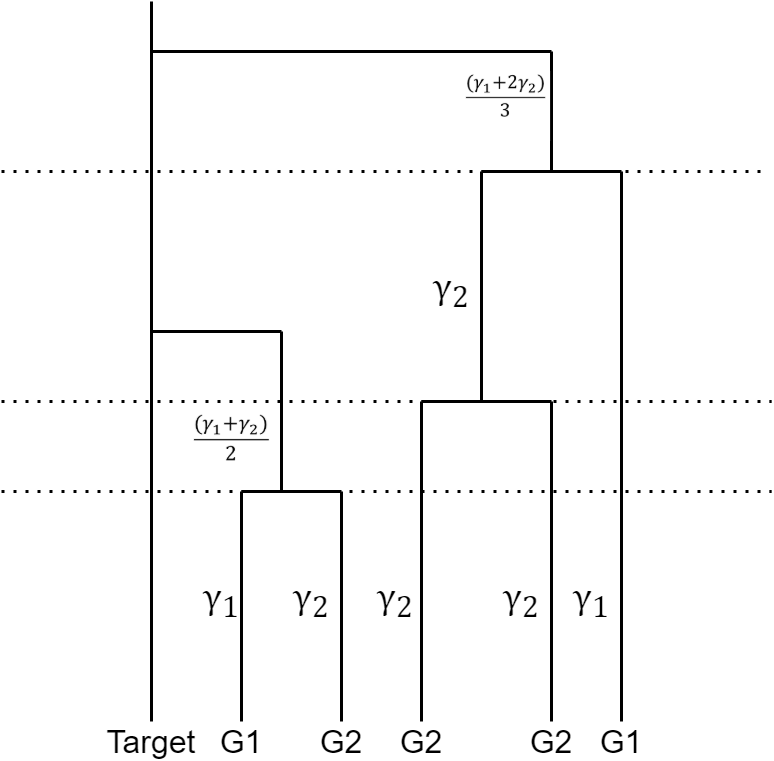
\includegraphics[scale=0.275]{figures/ghost buster simon myers-Page-1.png}
    \caption{Toy example showing how coalescence rates depends on the weighted sum of coalescence rates of the descendants}
    \label{fig1}
\end{figure}

The MLE of coalescence rates derived in section \ref{sec:ch1-gb-theory} also assumes independence of trees along the genome. To address this, we employ a Hidden Markov Model (HMM) to capture ancestry switches along the genome, treating each location Markovian. This approach mitigates the independence assumption and enhances the power of our likelihood estimation further.

\subsubsection{Likelihood of a single coalescence event}

Under our model, the probability distribution of observing a single coalescence event at time $t$ can be expressed as follows:
\begin{equation}
    P(t | \gamma) = \frac{\sum_{g=1}^R\gamma_{g}(m)n_{g}}{\sum_{g=1}^R n_{g}}e^{-\sum_{g=1}^R \gamma_{g} \cdot O_{g}}
\end{equation}
where, $n_{g} =$ number of group $g$ individuals coalescing in the coalescence event, $\gamma_{g}(m)$ is the corresponding coalescence rate of group $g$ in time epoch $m$ and, $O_{g}$ is the opportunity and equal to the sum of branch length from lower epoch boundary to the coalescence event corresponding to all group g individuals coalescing at $t$. This weighting corresponds to choosing which group to coalesce at a given coalescence event based on the proportion of descendants belonging to that particular group in that coalescence event. 

\subsection{EM derivation: the likelihood}
\subsubsection{Terminology}
\label{terminology}
We aim to fit a mixture model to cluster the genome based on variations in coalescence rates. To reduce computational costs, we divide the genome into $T$ small grids and focus on inferring local ancestry at these grid points, rather than at every individual location on the genome. Additionally, we approximate coalescence rates as piecewise constant functions over time, defined by $E$ time epochs that are equally spaced on a logarithmic scale. For the derivation of the EM algorithm, we use the following terminology:
\begin{itemize}    
    \item Our input data are the genealogies which contain:
    \begin{enumerate}
        \item $Q_l =$ Number of coalescence events with the target in $l^{th}$ grid
        \item $e_{li} =$ Epoch in which $i^{th}$ coalescent event happens in the $l^{th}$ grid
        \item $t_{li} =$ Coalescence time for the $i^{th}$ coalescence event in the $l^{th}$ grid
        \item $r_{l} =$ Genomic distance between $(l-1)^{th}$ and $l^{th}$ position along the genome
    \end{enumerate}

    \item The parameters we infer using are EM algorithm are:
    \begin{enumerate}
        \item $\gamma_{jg}(m) =$ Coalescence rate between reference group $g$ and the target in the $j^{th}$ mixture component and in epoch $m$
        \item $\pi_j  = P(z_l = j) =$ Cluster proportion of the $j^{th}$ mixture component
        \item $\lambda =$ Admixture time in generations 
    \end{enumerate}

    \item Lets define some fixed constants we will use in derivation:
    \begin{enumerate}
        \item $C =$ Total number of coalescence events in the ARG
        \item $T =$ Total number of grid points
        \item $A =$ Number of clusters assumed in the target
        \item $N_{li} =$ Number of reference individuals in $i^{th}$ coalescence event and $l^{th}$ grid
        \item $E =$ Number of time epochs (where the coalescence rates are assumed piece-wise constant)
    \end{enumerate}

    \item We will maintain consistency by using the same subscript to index the same variables throughout the derivation:
    \begin{enumerate}
        \item $l =$ Grid position along the genome
        \item $i =$ Coalescence event count
        \item $g =$ Pre-defined reference groups (e.g. Papuans, Denisovans, etc.)
        \item $j =$ Cluster or component in the mixture
        \item $e =$ Time epoch going backwards in time
    \end{enumerate}

    \item In the E-step, we introduce hidden variables to facilitate analytical updates. These variables are probabilistically inferred based on the current estimates of the parameters:
    \begin{enumerate}
        \item $z_l =$ Local ancestry of the target at position $l$
        \item $q_{li} =$ Reference individual index that coalesces in the $i^{th}$ coalescence event and $l^{th}$ grid
        \item $\omega_l =$ Number of recombinations since admixture between position $l-1$ and $l$
    \end{enumerate}

\end{itemize}

\subsubsection{The ``true'' likelihood}
We wish to formalize the likelihood for the mixture model described verbally in section \ref{the_model}. We write the likelihood of the mixture model as the product over all coalescence events with the target lineage in the ancestral recombination graph (ARG): 
\begin{equation}
    P (t,z,q \vert \gamma, \pi, \lambda) = \prod_{c=1}^{C} \prod_{j = 1}^A \prod_{g =1}^{R} \prod_{m = 1}^E P (t_c,z_c = j,q_c=g \vert \gamma, \pi, \lambda)^{I_{\{z_c = j\}} I_{\{q_c = g\}} I_{\{e_c = m\}}}
\label{true_likelihood1}
\end{equation}

Where, $t$ is the vector of observed coalescence times, $z$ and $q$ are hidden variables per coalescence event. It is important to note the coalescence events in a ARG can span more than one tree, especially branches lower in the tree are less likely to be affected due to recombination and thus last longer along the genome. Next, we introduce windowing the genome and appropriately scaling the likelihood to still get the above equation as follows:
\begin{equation}
    \footnotesize
    P(t,z,q \vert \gamma, \pi, \lambda) = \prod_{c=1}^{C} \prod_{j = 1}^A \prod_{g =1}^{R} \prod_{m = 1}^E \prod_{l =1}^{T} \left( P(t_c,z_c = j,q_c=g \vert \gamma, \pi, \lambda)^{I_{\{z_c = j\}} I_{\{q_c = g\}} I_{\{e_c = m\}}} \right) ^{\frac{I_{\{w_c = l\}}}{K_c}}
\label{true_likelihood2}
\end{equation}
where, $I_{\{w_c = l\}}$ is the indicator random variable indicating if the $l^{th}$ grid point overlaps with the branch corresponding to $c^{th}$ coalescence event, and $K_c$ is the total number of grids the branch corresponding to $c^{th}$ coalescence event lasts (we refer to this term as node persistence). We scale the likelihood in equation \ref{true_likelihood2} by $\frac{1}{K_c}$ such that it is still equal to the original likelihood in equation \ref {true_likelihood1}. 

\subsubsection{Accounting for uncertain coalescence events}

Genealogies inferred from genetic variation data come with the added complexity of uncertainty, as they are not always entirely accurate. The support for a particular node in the tree is stronger when there is a mutation mapped just above that node. To account for this uncertainty, we scale the likelihood by the confidence in each coalescence event. Specifically, as we move backward in time along the target lineage, we count the number of coalescence events that occur before encountering a mutation. All coalescence events between successive mutations are then weighted by one divided by the number of such events, effectively treating them as a single coalescence event. This adjustment improves the robustness of our method to errors in inferred genealogies, as demonstrated in empirical analyses. Overall this results in scaling the likelihood in equation \ref{true_likelihood2} by an additional term, $H_c$, which calculates the effective contribution of a coalescence event to the likelihood depending on its certainty. The updated likelihood is now given as: 
\begin{equation}
    \footnotesize
    P(t,z,q \vert \gamma, \pi, \lambda) = \prod_{c=1}^{C} \prod_{j = 1}^A \prod_{g =1}^{R} \prod_{m = 1}^E \prod_{l =1}^{T} \left( P(t_c,z_c = j,q_c=g \vert \gamma, \pi, \lambda)^{I_{\{z_c = j\}} I_{\{q_c = g\}} I_{\{e_c = m\}}} \right) ^{\frac{I_{\{w_c = l\}}}{B_c}}
\label{true_likelihood3}
\end{equation}
where, $B_c = \frac{H_c}{K_c}$ is the effective scaling factor accounting for branch persistence and certainty of coalescence events in inferred genealogies. Even though we divide the likelihood in different grids its not straight-forward to optimize the likelihood directly. In the next section, we approximate the likelihood in equation \ref{true_likelihood3} so that we can use Markov models for inference. 


\subsubsection{Markovian approximation to the ``true'' likelihood}
We perform a Markovian approximation to the ``true'' likelihood defined in equation \ref{true_likelihood3} and re-write the cluster membership $z$ in terms of window $l$ instead of coalescence event $c$. More formally we approximate as follows:
\begin{equation}
    P (t,z,q \vert \gamma, \pi, \lambda) \approx \prod_{l =1}^{T} \prod_{j = 1}^A \prod_{i = 1}^{Q_l} \prod_{k =1}^{N_{li}} \prod_{m = 1}^E \Big( P(t_{li}, q_{li} = k, z_l = j \vert \gamma, \pi, \lambda) ^ {I_{\{q_{l i} = k\}}  I_{\{e_{l i} = m\}}} \Big) ^{\frac{I_{\{z_l = j\}}}{B_{li}}}
    \label{markov_approx}
\end{equation}
where, $q_{li}$ is a hidden variable recording which reference individual the target coalesced with in the $i^{th}$ coalescence event at grid $l$. Similarly, $Q_{l}$ is the total number of coalescence events which overlap with grid point $l$ and $N_{li}$ is the list of reference individuals which coalesce at $q_{li}^{th}$ coalescence event. The Markovian assumption not only allows us to use markov models like HMMs for inference but also simplifies the cluster membership per position $l$ which can be easily interpreted as local ancestry at position $l$. We further simplify the equation \ref{markov_approx} and separate it into two parts.

\begin{equation}
    \footnotesize
    P (t,z,q \vert \gamma, \pi, \lambda) = \underbrace{P(z \vert \pi, \lambda)}_{\text{Term 2}} \prod_{l =1}^{T} \prod_{j = 1}^A \prod_{i = 1}^{Q_l} \prod_{k =1}^{N_{li}} \prod_{m = 1}^E \underbrace{\Big( P(t_{li}, q_{li} = k \vert z_l = j, \gamma) ^ {I_{\{q_{l i} = k\}}  I_{\{e_{l i} = m\}}} \Big) ^{\frac{I_{\{z_l = j\}}}{B_{li}}}}_{\text{Term 1}}
    \label{eq:term1_term2}
\end{equation}

We perform expectation-maximization and optimize term 1 to get the $\gamma$ (coalescence rates) and term 2 to get $\lambda$ (admixture time) and $\pi$ (global cluster proportions). In the following sections we simplify our calculations by deriving the EM updates for term 1 and term 2 separately. 

\subsection{EM derivation: inference of coalescence rates}
We write the likelihood term 1 in equation \ref{eq:term1_term2} which only depends on coalescence rates as follows: 
\begin{equation}
     P(t, q \vert z, \gamma) = \prod_{l = 1}^T \prod_{j = 1}^A \prod_{i = 1}^{Q_l} \prod_{k =1}^{N_{li}} \prod_{m = 1}^E   P(t_{li}, q_{l i} = k \vert z_l = j, \gamma) ^ {\frac{I_{\{z_l = j\}}I_{\{q_{l i} = k\}}  I_{\{e_{l i} = m\}}}{B_{li}}}
\label{eq:scaled_ll}
\end{equation}
where, The indicator random variables $I_{\{z_l = j\}}$, $I_{\{e_{l i} = m\}}$ and, $I_{\{q_{l i} = k\}}$ are present to simplify the equation when writing it down for all the trees and coalescence events in that tree. The log-likelihood is given by:

\begin{equation}
     \log P(t, z, q \vert \gamma) = \sum_{l = 1}^T \sum_{j = 1}^A \sum_{i = 1}^{Q_l} \sum_{k =1}^{N_{li}} \sum_{m = 1}^E  \frac{I_{\{q_{l i} = k\}} I_{\{z_l = j\}} I_{\{e_{l i} = m\}} \log P(t_{li}, q_{l i} = k \vert z_l = j, \gamma)}{B_{li}} 
\end{equation}

We can simplify the log-likelihood further as:
\begin{equation}
    P(q_{li} = k, t_{li} | z_l = j, \gamma ) = P(t_{li} | \gamma, z_l = j, q_{li} = k)P(q_{li} = k | z_l = j, \gamma)
\end{equation}

\begin{enumerate}
    \item Looking at the first term $P(t_{li} | \gamma, z_l = j, q_{li} = k)$:
\begin{align}
    P(t_{li} | \gamma, z_l = j, q_{li} = k) = P(t_{li} | \gamma, z_l = j) \nonumber \\
    P(t_{li} | \gamma, z_l = j) = \frac{\sum_{g=1}^R\gamma_{jg}(m)n_{lig}}{\sum_{g=1}^R n_{lig}}e^{-\sum_{g=1}^R \gamma_{jg} \cdot O_{lg}[i]}
\end{align}
where, $n_{lig} =$  number of group $g$ individuals coalescing in the $i^{th}$ coalescence event and position $l$ and, $O_{lg}[i] =$ sum of branch length from lower epoch boundary to the $i^{th}$ coalescence event corresponding to all group g individuals coalescing at $t_{li}$.
\vspace{3mm}
\item The second term $P(q_{li} = k | z_l = j, \gamma)$ simplifies to:
\begin{equation}
    P(q_{li} = k | z_l = j, \gamma) = \frac{\gamma_{jg(k)}(m)C_{ik}\sum_{g=1}^Rn_{lig}}{\sum_{g=1}^R \gamma_{jg}(m)n_{lig}}
\label{eq:qli}
\end{equation}

where, $g(k)$ means the group assignment (among $R$ groups) of the $k^{th}$ individual in the reference panel, and $C_{ik}$ is the contribution of $k^{th}$ individual in $i^{th}$ lineage. 
\end{enumerate}

Overall $P(q_{li} = k, t_{li} | z_l = j, \gamma )$ can be written as: 
\begin{align}
    P(q_{li} = k, t_{li} | \gamma, z_l = j ) = \gamma_{jg(k)}(m)C_{ik}e^{-\sum_{g=1}^R \gamma_{jg}\cdot O_{lg}[i]} \nonumber \\
    \propto \gamma_{jg(k)}(m)*e^{-\sum_{g=1}^R \gamma_{jg}\cdot O_{lg}[i]}
    \label{eq:likelihood}
\end{align}

We can maximize the likelihood corresponding to term 1 through an expectation-maximization algorithm. Where, in the E-step we define the expected log-likelihood of the data given the hidden variables and the previous estimates of the parameters (including $\lambda$ and $\pi$), and in the M-step we maximize this expected log-likelihood. Under the expectation maximization framework, it is guaranteed the likelihood is going to increase every iteration thereby guaranteeing convergence to a local minima. Next, we derive the E-step and M-step for our likelihood in equation \ref{eq:likelihood}.
 
\subsubsection{E-step}

In the E-step we calculate the expected log-likelihood, where the expectation is w.r.t the hidden variables conditioned on the data and previous parameter estimation. We therefore proceed by stating the expected log-likelihood in our case:
\begin{equation}
   E_{z, q | \gamma^{t-1}, \lambda^{t-1}, \pi^{t-1}, t} \Big(  \sum_{l = 1}^T \sum_{j = 1}^A \sum_{i = 1}^{Q_l} \sum_{k =1}^{N_{li}} \sum_{m = 1}^E  \frac{I_{\{q_{l i} = k\}} I_{\{z_l = j\}} I_{\{e_{l i} = m\}} \log P(t_{li}, q_{l i} = k \vert z_l = j, \gamma)}{B_{li}} \Big)
 \end{equation}

We start simplifying the expected log-likelihood by taking the expectation inside the summation, and transforming the expected value of indicator random variables as probabilities.  
\begin{footnotesize}
\begin{align}
    &= \sum_{l = 1}^T \sum_{j = 1}^A  \sum_{i = 1}^{Q_l} \sum_{k =1}^{N_{li}} \sum_{m = 1}^E P(q_{li} = k, z_l = j \mid \gamma^{t-1}, \lambda^{t-1}, \pi^{t-1}, t) I_{\{e_{l i} = m\}} \frac{\log(P(q_{l i} = k, t_{li} \mid z_l = j, \gamma ))}{B_{li}}
\end{align}
\end{footnotesize}

Simplifying further and substituting the value of $log(P( q_{l i} = k, t_{li} | z_l = j, \gamma ))$ from equation \ref{eq:likelihood}. Note, we omit the constants of proportionality as they do not depend on the coalescence rates and thus will not affect the maximization in the M-step.
\begin{align}
    &= \sum_{l = 1}^T \sum_{j = 1}^A \sum_{i = 1}^{Q_l} \sum_{k = 1}^{N_{li}} \sum_{m = 1}^E \Bigg( 
        P(q_{li} = k \mid \gamma^{t-1}, t, z_l = j) P(z_l = j \mid t, \gamma^{t-1}, \lambda^{t-1}, \pi^{t-1}) \nonumber \\
    &\quad \times I_{\{e_{l i} = m\}} \frac{\log(P(q_{l i} = k, t_{li} \mid z_l = j, \gamma))}{B_{li}} \Bigg) \nonumber \\
    &= \sum_{l = 1}^T \sum_{j = 1}^A \sum_{i = 1}^{Q_l} \sum_{k = 1}^{N_{li}} \sum_{m = 1}^E \Bigg( 
        P(q_{li} = k \mid \gamma^{t-1}, t, z_l = j) P(z_l = j \mid t, \gamma^{t-1}, \lambda^{t-1}, \pi^{t-1}) \nonumber \\
    &\quad \times I_{\{e_{l i} = m\}} \frac{\log(\gamma_{jg(k)}(m)) - \sum_{g=1}^R \gamma_{jg} \cdot O_{lg}[i]}{B_{li}} \Bigg) 
\end{align}

Note the probability of $q_{li}$ (as defined in equation \ref{eq:qli}) does not depend on admixture time and proportion. We can simplify the expected log-likelihood further and switch the individual assignment hidden variable $q_{li}$ to more easily computable group assignment hidden variable $q'_{li}$. 
\begin{align}
   &\color{red}{\sum_{l = 1}^T \sum_{j = 1}^A \sum_{i = 1}^{Q_l} \sum_{k = 1}^{N_{li}} \sum_{m = 1}^E \Bigg( 
       P(q_{li} = k \mid \gamma^{t-1}, z_l = j) P(z_l = j \mid t, \gamma^{t-1}, \lambda^{t-1}, \pi^{t-1})} \nonumber \\
   &\quad \color{red}{\times I_{\{e_{l i} = m\}} \frac{\log(\gamma_{jg(k)}(m))}{B_{li}} \Bigg)} \nonumber \\
   &\color{blue}{- \sum_{l = 1}^T \sum_{j = 1}^A \sum_{i = 1}^{Q_l} \sum_{k = 1}^{N_{li}} \sum_{m = 1}^E \Bigg( 
       P(q_{li} = k \mid \gamma^{t-1}, z_l = j) P(z_l = j \mid t, \gamma^{t-1}, \lambda^{t-1}, \pi^{t-1})} \nonumber \\
   &\quad \color{blue}{\times I_{\{e_{l i} = m\}} \frac{\sum_{g=1}^R \gamma_{jg} \cdot O_{lg}[i]}{B_{li}} \Bigg)}
\end{align}

We group the individuals based on group assignment in the first term (red term) and use $\sum_{k =1}^{N_{li}} P(q_{li} = k | \gamma^{t-1}, z_l = j) = 1$ in the second term (blue term). 
\begin{align}
   &\color{red}{\sum_{l = 1}^T \sum_{j = 1}^A \sum_{i = 1}^{Q_l} \sum_{k = 1}^{N_{li}} \sum_{m = 1}^E \Bigg( 
       P(q'_{li} = g \mid \gamma^{t-1}, z_l = j) P(z_l = j \mid t, \gamma^{t-1}, \lambda^{t-1}, \pi^{t-1})} \nonumber \\
   &\quad \color{red}{\times I_{\{e_{l i} = m\}} \frac{\log(\gamma_{jg}(m))}{B_{li}} \Bigg)} \nonumber \\
   &\color{blue}{- \sum_{l = 1}^T \sum_{j = 1}^A \sum_{i = 1}^{Q_l} \sum_{m = 1}^E \Bigg( 
       P(z_l = j \mid t, \gamma^{t-1}, \lambda^{t-1}, \pi^{t-1}) I_{\{e_{l i} = m\}}}  \sum_{g=1}^R \frac{\gamma_{jg} \cdot O_{lg}[i]}{B_{li}} \Bigg)
   \label{estep:ell-simple}
\end{align}

Lets denote $U_{l,i,g,j,m}^{t-1}$ as the first term corresponding to the membership ``group g individual coalesces in the $i^{th}$ coalescence event''. And, lets denote $T_{l,j}^{t-1}$ as the second term corresponding to the local ancestry of the target. We use the forward-backward algorithm for HMM to evaluate $T_{l,j}$ in future section \ref{sec:term2_estep}. Whereas, we calculate $U_{l,i,g,j,m}^{t-1}$ based on our model as follows:
\begin{equation}
    U_{l,i,g,j,m}^{t-1} = P(q'_{li} = g | \gamma^{t-1}, z_l = j) = \frac{\gamma_{jg}^{t-1}(m)c_{lig}}{\sum_{g=1}^R \gamma_{jg}^{t-1}(m)c_{lig}}
    \label{estep:u}
\end{equation}
where, $c_{lig} = \frac{n_{lig}}{\sum_{g=1}^R n_{lig}}$ are the normalized proportions of coalescence count for each coalescence event

\subsubsection{M-step}

Once we have the expected log-likelihood we can maximize it in the M-step. We substitute $U_{l,i,g,j,m}^{t-1}$ and $T_{l,j}^{t-1}$ as hidden variables from equation \ref{estep:u} and HMM forward-backward into equation \ref{estep:ell-simple}. We Maximize w.r.t $\gamma_{jg}(m)$ as follows:
\begin{align}
    &\sum_{l = 1}^T \sum_{i = 1}^{Q_l} \sum_{j = 1}^A \sum_{g = 1}^R \sum_{m = 1}^E \Bigg( 
        U_{l,i,g,j,m}^{t-1} T_{l,j}^{t-1} I_{\{e_{l i} = m\}} \frac{\log(\gamma_{jg}(m))}{B_{li}} \Bigg) \nonumber \\
    &- \sum_{l = 1}^T \sum_{i = 1}^{Q_l} \sum_{j = 1}^A \sum_{m = 1}^E \Bigg( 
        T_{l,j}^{t-1} I_{\{e_{l i} = m\}} \sum_{g = 1}^R \frac{\gamma_{jg} \cdot O_{lg}[i]}{B_{li}} \Bigg)
\end{align}

Differentiating w.r.t $\gamma_{jg}(m)$ and setting it to 0 we get:
\begin{equation}
\sum_{l = 1}^T \sum_{i = 1}^{Q_l}  \Big( \frac{I_{\{e_{l i} = m\}}U_{l,i,g,j,m}^{t-1} T_{l,j}^{t-1}}{\gamma_{jg}(m)B_{li}} \Big) -  \sum_{l = 1}^T \sum_{i = 1}^{Q_l} \Big(\frac{I_{\{e_{l i} = m\}} T_{l,j}^{t-1}  O_{lg}[i]}{B_{li}} \Big) = 0
\end{equation} 

% \begin{equation}
% \sum_{l = 1}^T \sum_{i = 1}^{Q_l}  \Big( \frac{I_{\{e_{l i} = m\}}U_{l,i,g,j,m}^{t-1} T_{l,j}^{t-1}}{\gamma_{jg}(m)} \Big) =  \sum_{l = 1}^T \sum_{i = 1}^{Q_l} \Big(I_{\{e_{l i} = m\}} T_{l,j}^{t-1}  O_{lg}[i] \Big)
% \end{equation} 
\begin{align}
    \gamma_{jg}^{t}(m) &= \frac{\sum_{l = 1}^T \sum_{i = 1}^{Q_l}  I_{\{e_{l i} = m\}} U_{l,i,g,j,m}^{t-1} T_{l,j}^{t-1}/B_{li}}{\sum_{l = 1}^T \sum_{i = 1}^{Q_l}  I_{\{e_{l i} = m\}} T_{l,j}^{t-1}  O_{lg}[i]/B_{li} } \nonumber \\
    \gamma_{jg}^{t}(m) &= \frac{\sum_{l = 1}^T \sum_{i = 1}^{Q_l}  I_{\{e_{l i} = m\}} \frac{\gamma_{jg}^{t-1}(m)c_{lig}}{\sum_{g=1}^R \gamma_{jg}^{t-1}(m)c_{lig}} T_{l,j}^{t-1}/B_{li}}{\sum_{l = 1}^T \sum_{i = 1}^{Q_l}  I_{\{e_{l i} = m\}} T_{l,j}^{t-1}  O_{lg}[i]/B_{li} }
\label{eq:gamma_update}
\end{align}
where, $Opp_{lg}(m)$ is the sum of branch length in epoch $m$. It is important to note we do not need to store $U_{l,i,g,j,m}^{t-1}$ explicitly, we can instead store $\gamma^{t-1}$ to save memory.

\subsection{EM derivation: inference for admixture time \& proportions}
% \textbf{Simplifying the log-likelihood of term 2} 

We assume a markov model to write the likelihood for term 2 in equation \ref{eq:term1_term2}. Apart from the local ancestry hidden variable ($z$) we also introduce another hidden variable, $\omega_l$ to record the number of recombination events since admixture between $l-1$ and $l$. We assume a user-defined recombination map is available, reporting distance between two grid points in genomic position as $r_l$. The likelihood of the term can then be written as follows:
\begin{equation}
    P(z, \omega_l \vert \lambda, \pi) \propto \prod\limits_{l=1}^{T} \Big( \prod\limits_{j=1}^{A} \pi_j ^ {I\{z_l = j\} I\{\omega_l > 0\}} \Big) (\lambda r_l)^{\omega_l} e^{-\lambda r_l}
\end{equation}
where, $z_l$ is local ancestry at position $l$, $\omega_l$ is the hidden variable recording the number of recombinations between site $l-1$ and $l$ since the admixture time and $r_l$ is the user-defined recombination rate at position $l$. The likelihood for the number of recombinations is given by a Poisson counting process. It is important to note, the local ancestry change happens if there is atleast a recombination event. The parameters of the model are $\lambda$, which is the admixture time and $\pi$ which are the global cluster proportions. The log-likelihood can be written as follows:
\begin{equation}
    \log P(z, \omega_l \vert \lambda, \pi) = \sum\limits_{l=1}^{T} \Big( \sum\limits_{j=1}^{A} I\{z_l = j\} I\{\omega_l > 0\} \log \pi_j \Big) + \omega_l \log \lambda r_l - \lambda r_l + \text{constants}
\end{equation}

\subsubsection{E-step}
\label{sec:term2_estep}

In order to perform EM, we look at the expected log-likelihood of the data where the expectation is taken with respect to the hidden variables conditioned on the data (coalescence times with the target) and previous iteration's model parameters (including the $\gamma$).
\begin{equation}
    E_{z, \omega_l \vert \gamma^{t-1}, \lambda^{t-1}, \pi^{t-1}, t}\Big( \sum\limits_{l=1}^{T} \Big( \sum\limits_{j=1}^{A} I\{z_l = j\} I\{\omega_l > 0\} \log \pi_j \Big) + \omega_l \log \lambda r_l - \lambda r_l \Big)
\end{equation}

We start simplifying the expected log-likelihood by taking the expectation inside the summation, and transforming the expected value of indicator random variables as probabilities. 
\begin{equation}
     \sum\limits_{l=1}^{T} \Big( \sum\limits_{j=1}^{A} P(z_l = j, \omega_l > 0 \vert \gamma^{t-1}, \lambda^{t-1}, \pi^{t-1}, t) \log \pi_j \Big) + E(\omega_l) log \lambda r_l - \lambda r_l
\end{equation}

where, the expectation is taken over the hidden variables conditioned on the data and previous iterations' parameter updates. We are interested to infer three terms, (1) $P(z_l = j, \omega_l > 0)$, (2) $E(\omega_l)$ and (3) $P(z_l = j | t, \gamma^{t-1}, \lambda^{t-1}, \pi^{t-1})$. We start with the first term:
\begin{align}
    P&(z_l = j, \omega_l > 0 \vert P^{t-1}, t) = P(z_l = j \vert P^{t-1}, t) P(\omega_l > 0 \vert z_l = j, P^{t-1}, t) \nonumber \\
    &= P(z_l = j \vert P^{t-1}, t) \sum\limits_{i=1}^{A} P(\omega_l > 0 \vert z_l = j, z_{l-1} = i, P^{t-1}, t) P(z_{l-1} = i \vert z_l = j, P^{t-1}, t) \nonumber \\
    &= \sum\limits_{i=1}^{A} P(z_l = j \vert P^{t-1}, t) P(\omega_l > 0 \vert z_l = j, z_{l-1} = i, P^{t-1}, t) P(z_{l-1} = i \vert z_l = j, P^{t-1}, t) \nonumber \\
    &= \sum\limits_{i=1}^{A} \color{red}{P(\omega_l > 0 \vert z_l = j, z_{l-1} = i, P^{t-1})} \color{blue}{P(z_l = j, z_{l-1} = i \vert P^{t-1}, t)}
\label{eq:hmm_estep}
\end{align}
where, $P^{t-1} = (\gamma^{t-1}, \lambda^{t-1}, \pi^{t-1})$ is a short-hand for the tuple of all previous parameters. We denote the second term (coloured in blue) as $\epsilon_{ij}(l)$ as it denotes the probability of being in state $i$ and state $j$ at position $l-1$ and $l$ respectively. Similar to the Baum-Welch algorithm we can solve for $\epsilon_{ij}(l)$ through the forward backward pass in hidden markov models. 

\begin{footnotesize}
\begin{align}
    &\epsilon_{ij}(l) =P(z_l = j, z_{l-1} = i \vert P^{t-1}, t) \nonumber \\
    &= \frac{P(z_l = j, z_{l-1} = i, t \vert P^{t-1})}{P(t \vert P^{t-1})} \nonumber \\
    &= \frac{P(t_1 .., t_{l-1}, z_{l-1}=i \vert P^{t-1}) P(z_l=j \vert z_{l-1}=i, P^{t-1}) P(t_{l} .., t_T \vert z_l=j, P^{t-1}) P(t_l \vert z_l, P^{t-1})}{P(t \vert P^{t-1})} \nonumber \\
    &= \frac{P(t_1 .., t_{l-1}, z_{l-1}=i \vert P^{t-1}) P(z_l=j \vert z_{l-1}=i, P^{t-1}) P(t_{l} .., t_T \vert z_l=j, P^{t-1}) P(t_l \vert z_l, P^{t-1})}{\sum\limits_{j=1}^{A}\sum\limits_{i=1}^{A} P(t_1 .., t_{l-1}, z_{l-1}=i \vert P^{t-1}) P(z_l=j \vert z_{l-1}=i, P^{t-1}) P(t_{l} .., t_T \vert z_l=j, P^{t-1}) P(t_l \vert z_l, P^{t-1})}
\label{eq:epsilon_ij}
\end{align}
\end{footnotesize}
where, $P(t_1 .., t_{l-1}, z_{l-1}=i \vert P^{t-1})$ is called the forward-pass and $P(t_{l} .., t_T \vert z_l=j, P^{t-1})$ is called the backward-pass. The transition probability for the HMM is given as follows:
\begin{equation}
     P(z_l=j \vert z_{l-1}=i, P^{t-1}) = \begin{cases} (1 - e^{-r_l \lambda^{t-1}})\pi_j^{t-1}, & \text{if } i \neq j \\ e^{-r_l \lambda^{t-1}} + (1 - e^{-r_l \lambda^{t-1}})\pi_j^{t-1} , & \text{if } i = j \end{cases}
\end{equation}

Whereas the emission probability for the HMM $P(t_l \vert z_l, P^{t-1})$ only depends on $\gamma^{t-1}$ and follows from the scaled likelihood in equation \ref{eq:scaled_ll}:
\begin{equation}
   P(t_l \vert z_l, P^{t-1}) =  \Big( \frac{\sum_{g=1}^R\gamma^{t-1}_{jg}(m)n_{lig}}{\sum_{g=1}^R n_{lig}}e^{-\sum_{g=1}^R \gamma^{t-1}_{jg} \cdot O_{lg}[i]} \Big)^{\frac{1}{B_{li}}}
\end{equation}

The first term (red coloured) in equation \ref{eq:hmm_estep} can be thought as the probability of atleast one recombination event conditioned on local ancestry around it being $z_{l-1}$ and $z_l$. It is given as follows:
\begin{equation}
  P(\omega_l > 0 \vert z_l = j, z_{l-1} = i, P^{t-1}) = \begin{cases} 1, & \text{if } i \neq j \\ \frac{(1 - e^{-r_l \lambda^{t-1}})\pi_j^{t-1}}{e^{-r_l \lambda^{t-1}} + (1 - e^{-r_l \lambda^{t-1}})\pi_j^{t-1}} , & \text{if } i = j \end{cases}
\label{eq:e_of_recomb>0}
\end{equation}

The next term which needs to be calculated in the E-step is $E(\omega_l)$ where the expectation is with respect to the hidden variables $z_l, \omega_l$ conditioned on the data and previous iteration's model parameters. We can simplify the expectation as follows:
\begin{align}
    E(\omega_l \vert P^{t-1}, t) &= E(\omega_l \vert \omega_l > 0, P^{t-1}, t) P( \omega_l > 0 \vert P^{t-1}, t) \nonumber \\
    &= E(\omega_l \vert \omega_l > 0, P^{t-1}) P( \omega_l > 0 \vert P^{t-1}, t) \nonumber \\
    &= \frac{\lambda^{t-1}r_l}{1 - e^{-\lambda^{t-1}r_l}} P( \omega_l > 0 \vert P^{t-1}, t)
\label{eq:estep_121}
\end{align}
where, $P^{t-1} = (\gamma^{t-1}, \lambda^{t-1}, \pi^{t-1})$ is a short-hand for the tuple of all previous parameters. In order to evaluate $ P( \omega_l > 0 \vert P^{t-1}, t)$ we do the following: 
\begin{align}
  P( \omega_l > 0 \vert P^{t-1}, t) &= \sum\limits_{j=1}^{A}\sum\limits_{j=1}^{A}  P( \omega_l > 0 \vert z_l = j, z_{l-1} = i, P^{t-1}, t) P(z_l = j, z_{l-1} = i \vert P^{t-1}, t) \nonumber \\
  &= \sum\limits_{j=1}^{A}\sum\limits_{j=1}^{A}  P( \omega_l > 0 \vert z_l = j, z_{l-1},  P^{t-1} = i) \epsilon_{ij}(l)
\label{eq:e_of_recomb}
\end{align}

We have already calculated the terms needed in equation \ref{eq:e_of_recomb} before in equation \ref{eq:epsilon_ij} and \ref{eq:e_of_recomb>0}. Lastly to calculate the local ancestry estimate $P(z_l = j | t, \gamma^{t-1}, \lambda^{t-1}, \pi^{t-1})$ needed in equation \ref{eq:gamma_update} we perform a forward-backward pass:
\begin{equation}
    P(z_l = j | t, \gamma^{t-1}, \lambda^{t-1}, \pi^{t-1}) = \frac{P(t_1 .., t_{l-1}, z_{l-1}=i \vert P^{t-1})P(t_{l} .., t_T \vert z_l=j, P^{t-1})}{\sum\limits_{j=1}^{A}P(t_1 .., t_{l-1}, z_{l-1}=i \vert P^{t-1})P(t_{l} .., t_T \vert z_l=j, P^{t-1})}
\label{eq:hmm_forward_backward}
\end{equation}
where, $P(t_1 .., t_{l-1}, z_{l-1}=i \vert P^{t-1})$ and $P(t_{l} .., t_T \vert z_l=j, P^{t-1})$ is the forward and backward probability respectively. 

\subsubsection{M-step}

Once we know all the necessary equations in E-step we proceed to maximize the expected log-likelihood in M-step. We maximize w.r.t $\lambda$ and cluster proportions $\pi$ by maximizing the equation below: 
\begin{equation}
    \sum\limits_{l=1}^{T}  \color{red}{ \Big( \sum\limits_{j=1}^{A} P(z_l = j, \omega_l > 0 \vert \gamma^{t-1}, \lambda^{t-1}, \pi^{t-1}, t) \log \pi_j} \Big) + \color{blue}{E(\omega_l) log \lambda r_l - \lambda r_l }
\end{equation}

\begin{enumerate}
    \item Differentiating w.r.t $\pi_j$ and setting to zero we get:  
    \begin{align}
        \pi^{t}_j &\propto \sum\limits_{l=1}^{T} P(z_l = j, \omega_l > 0 \vert \gamma^{t-1}, \lambda^{t-1}, \pi^{t-1}, t) \nonumber \\
        \pi^{t}_j &= \frac{\sum\limits_{l=1}^{T} P(z_l = j, \omega_l > 0 \vert \gamma^{t-1}, \lambda^{t-1}, \pi^{t-1}, t)}{\sum\limits_{j=1}^{A} \sum\limits_{l=1}^{T} P(z_l = j, \omega_l > 0 \vert \gamma^{t-1}, \lambda^{t-1}, \pi^{t-1}, t)}
    \label{eq:pi_updates}
    \end{align}
    
    We get the term $P(z_l = j, \omega_l > 0 \vert \gamma^{t-1}, \lambda^{t-1}, \pi^{t-1}, t)$ from the E-step equation \ref{eq:hmm_estep}. 
    \item Differentiating w.r.t $\lambda$ and setting to zero we get:
    \begin{equation}
        \lambda^t = \frac{\sum\limits_{l=1}^{T}E(\omega \vert \gamma^{t-1}, \lambda^{t-1}, \pi^{t-1}, t)}{\sum\limits_{l=1}^{T}r_l}
    \label{eq:lambda_updates}
    \end{equation}
    
    Note we get the expected number of recombinations from equation \ref{eq:estep_121} in E-step.
    
\end{enumerate}

\clearpage

\subsection{Summary of the algorithm}
We present a summary of the EM algorithm for GhostBuster here:

\begin{algorithm}
\caption{EM Algorithm for GhostBuster}
\begin{algorithmic}[1]
\State \textbf{Input:} Geneologies $\mathbf{X} = \{(t_1,n_1), (t_2,n_2), \dots, (t_C,n_C)\}$ containing coalescence times and population counts for each coalescence event, number of components $A$, number of time epochs $E$, number of grid points $T$, total number of coalescence events $C$ and $R$ is the number of reference groups.
\State \textbf{Preprocessing:} Calculate likelihood scaling term $B_c$ for each coalescence event $c = 1, 2, \dots, C$, and $r_l$ genetic distance between two grid points
\State \textbf{Initialize:} Coalescence rates $\gamma_j^{(0)}$, mixing coefficients $\pi_j^{(0)}$ for each component $j = 1, 2, \dots, A$ and admixture time $\lambda^{(0)}$ 
\State \textbf{Set:} Iteration $t = 0$

\Repeat

    \State \textbf{E-step:} 
    
    \For{each component $j = 1, 2, \dots, A$}

    \For{each data point $(t_{li}, n_{li})$}
    
            \Comment{$t_{li}$ represent the coalescence time in $l^{th}$ grid and $i^{th}$ coalescence event}
            
            \Comment{$t_{li}$ represent the coalescence time in $l^{th}$ grid and $i^{th}$ coalescence event}
            
            \Comment{$P^{t-1} = \{\gamma^{t-1}, \lambda^{t-1}, \pi^{t-1}\}$}

            \vspace{2mm}
            
            \State Compute the likelihood under the component:
            \[
               P(t_l \vert z_l, P^{t-1}) =  \Big( \frac{\sum_{g=1}^R\gamma^{t-1}_{jg}(m)n_{lig}}{\sum_{g=1}^R n_{lig}}e^{-\sum_{g=1}^R \gamma^{t-1}_{jg} \cdot O_{lg}[i]} \Big)^{\frac{1}{B_{li}}}
            \]
        \EndFor
        
        \State Perform forward-backward pass with the HMM to get $P(z_l = j | X, P^{t-1})$ 

        \hspace{7mm} see equation \ref{eq:hmm_forward_backward}

        
    \EndFor
    
    \State \textbf{M-step:}
    \For{each component $k = 1, 2, \dots, A$}
        \State Update the coalescence rates:
        
        \hspace{7mm} see equation \ref{eq:gamma_update}

        \State Update the mixing coefficient:
        
        \hspace{7mm} see equation \ref{eq:pi_updates}
        
        \State Update the admixture time:
        
        \hspace{7mm} see equation \ref{eq:lambda_updates}
            
    \EndFor
    
    % \State \textbf{Compute:} Log-likelihood:
    % \[
    % \mathcal{L}^{(t+1)} = \sum_{i=1}^{N} \log \left( \sum_{k=1}^{K} \pi_k^{(t+1)} \mathcal{N}(x_i \mid \mu_k^{(t+1)}, \Sigma_k^{(t+1)}) \right)
    % \]

    % \State \textbf{Check for convergence:} If $|\mathcal{L}^{(t+1)} - \mathcal{L}^{(t)}| < \epsilon$, stop.
    \State \textbf{Increment:} $t = t + 1$
    
\Until{convergence}

\State \textbf{Output:} Final parameters $\{\gamma^{t}, \lambda^{t}, \pi^{t}\}$ for $k = 1, 2, \dots, A$

\end{algorithmic}
\end{algorithm}

\section{Method description}
\label{sec:ch2-gb-method}
\subsection{Overview of the method}

GhostBuster is a mixture model that clusters local trees in the genealogy based on coalescence rates between target lineage and a set of reference populations.
%
It relies on the assumption that an admixture or gene-flow event can be well characterized by these coalescence rates with reference populations.  
%
GhostBuster uses the genealogies inferred using large-scale genealogy inference softwares like Relate \cite{speidel2019method} directly and fits the mixture model using an iterative expectation maximization (EM) algorithm.
%
For this manuscript we restrict ourselves to Relate due to its scalability to thousands of samples and higher accuracy compared to other genealogy inference methods \cite{brandt2022evaluation}, but there is no conceptual difference in using our method with other genealogy inference methods.

The algorithm starts with a fixed number of mixture components (which is user-specified) and randomly initializing the admixture time and per-component genome-wide proportions and coalescence rates. 
%
The proportions are enforced to sum to one, whereas the coalescence rates are calculated with each reference population as a piece-wise constant function of time. 
%
In the E-step, GhostBuster calculates the expected log-likelihood of the data (in our case the coalescence time with reference individuals) conditioned on the local tree topology and previous estimates of the model parameters (proportions, admixture time and coalescence rates). 
%
We then use a hidden Markov model (HMM) to infer the local ancestry of the target individual.
%
The emissions for the HMM are modelled using the likelihood of the coalescence times, whereas the transitions are modelled using a Poisson process depending on recombination rates. 

In the M-step, we maximize the expected log-likelihood calculated in the E-step to get a new estimate of the model parameters. 
%
Under the EM algorithm, we are guaranteed this leads to non-decreasing likelihood updates and therefore a local optima \cite{dempster1977maximum}. 
%
The likelihood we derive conditions on the tree topology by carefully counting lineage contribution based on its descendants and leads to a higher statistical power to detect admixture events in our analysis, as we do not assume reference individuals are independent or use any composite likelihood assumptions.
%
A more detailed proof of the likelihood and the EM algorithm updates can be found in section \ref{sec:ch2-gb-theory}. 

A graphic overview of the method can be found in Figure \ref{fig:gb_overview}.

\begin{figure}[h!]
    \centering
    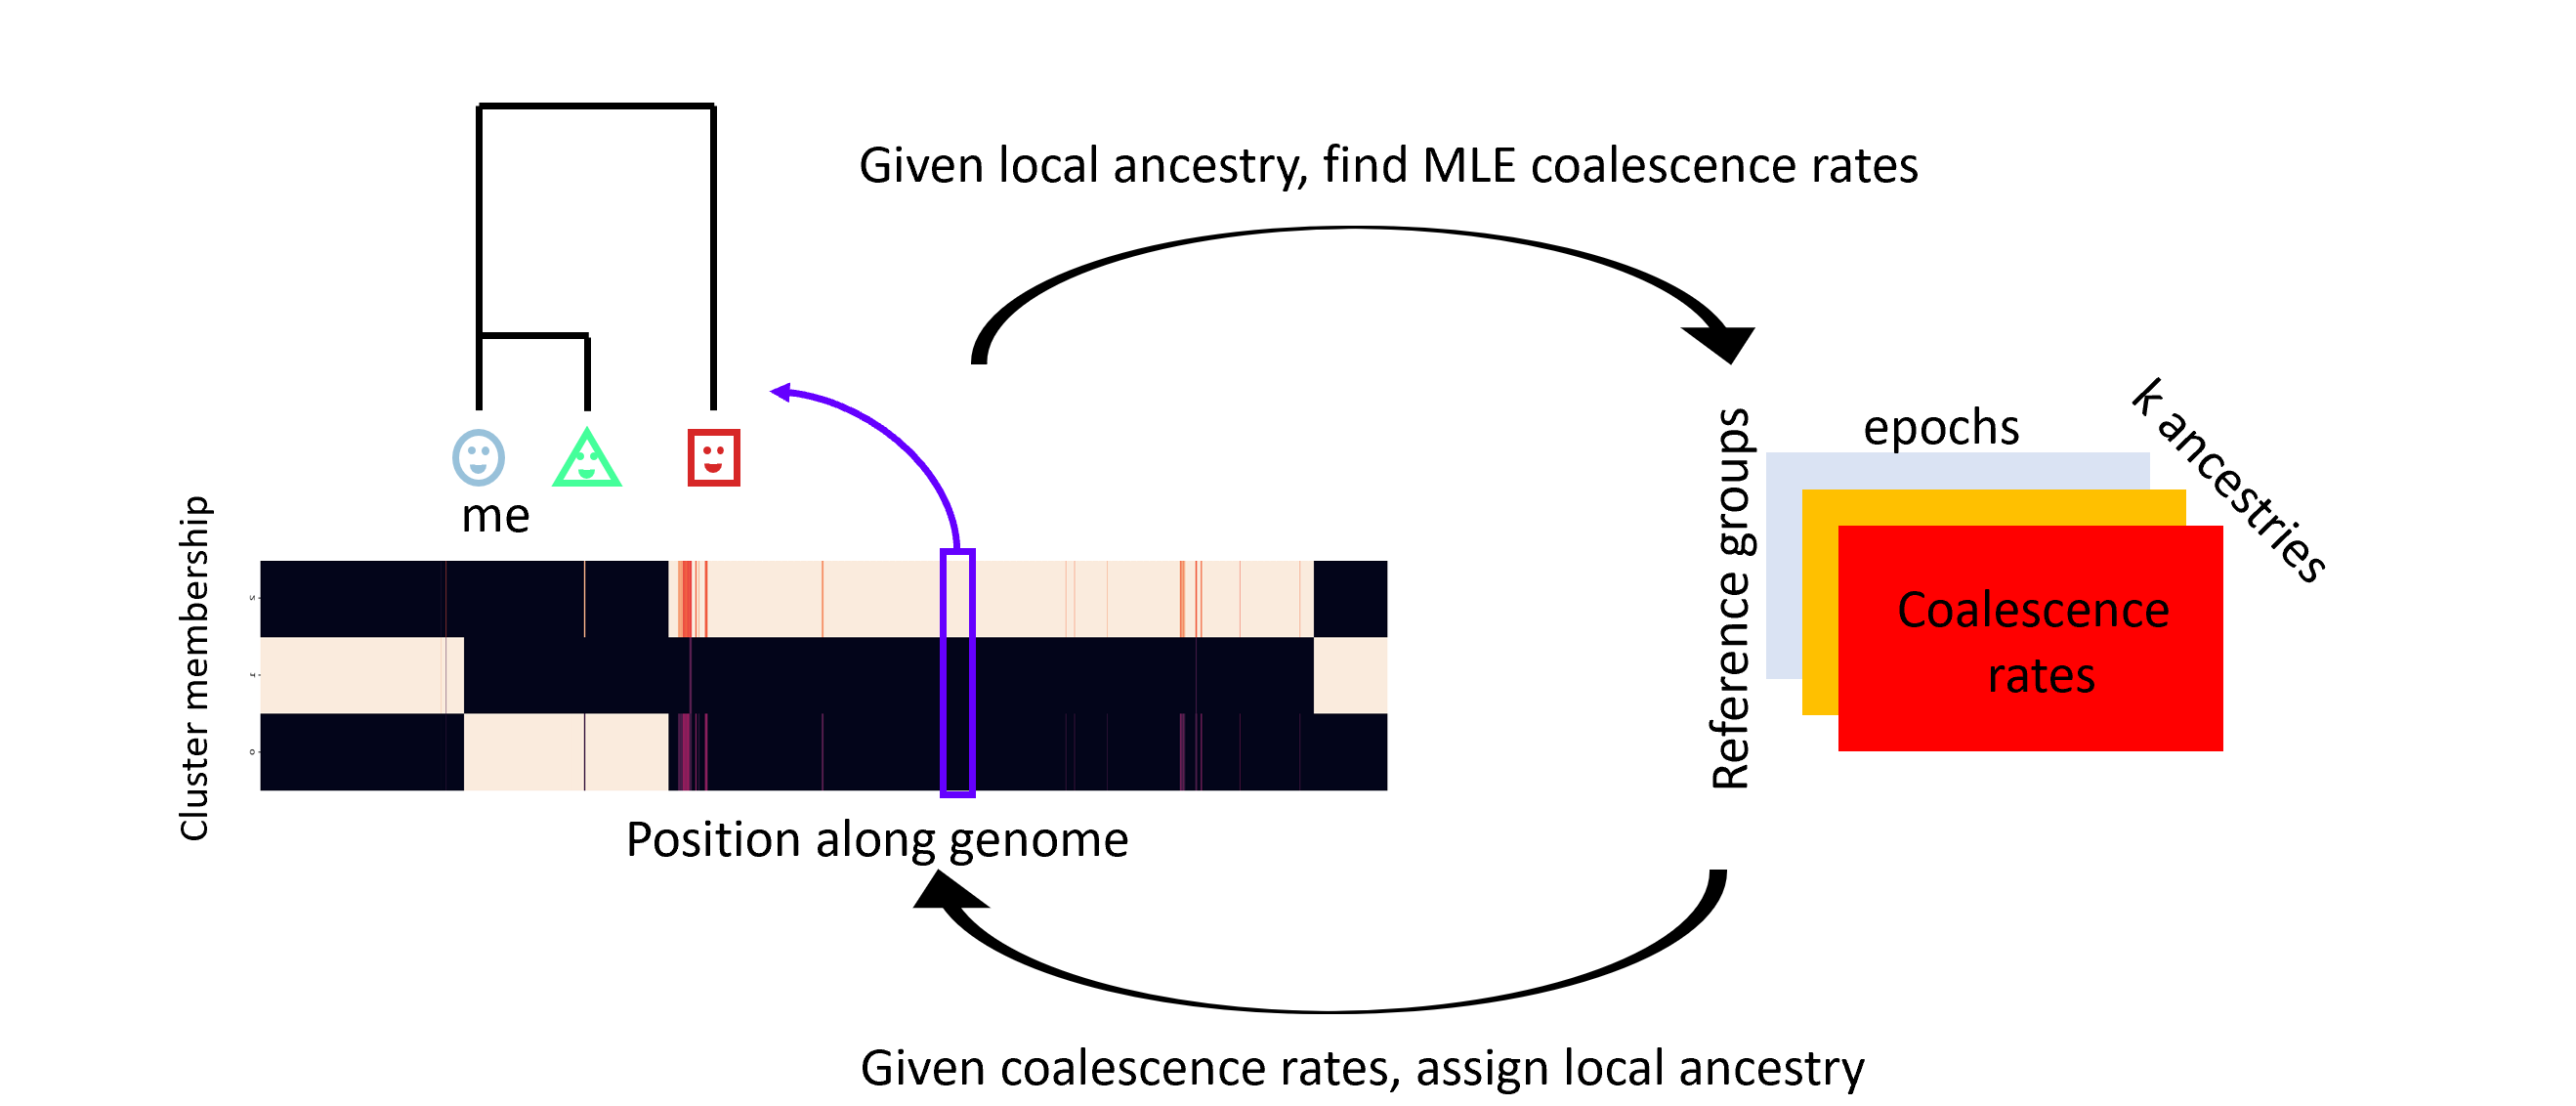
\includegraphics[scale=0.5]{figures/ghostbuster_method.PNG}
    \caption{\textbf{Overview of the GhostBuster algorithm.} The EM algorithm clusters the trees iteratively by successively updating the local ancestry given the coalescence rates in the E-step, and then the coalescence rates given the local ancestry in the M-step. }
    \label{fig:gb_overview}
\end{figure}


\subsection{PCA visualization to visualize ghost component}

To visualize the clustering of trees, we perform Principal Component Analysis (PCA) on the coalescence count and opportunity matrices obtained from the genealogies. The coalescence count matrix is an $N_{\text{ref}} \times N_{\text{tree}}$ matrix, where each entry $g,l$ represents the total contribution of reference group $g$ in the coalescence events at position $l$. In practice, we aggregate the contributions for all coalescence events occurring between predefined start and end time epochs, which typically correspond to the epochs used in the GhostBuster analysis. These epochs control the time periods in which we expect to observe differences in coalescence patterns. We construct a similar matrix for the opportunity, also an $N_{\text{ref}} \times N_{\text{tree}}$ matrix, where each entry $g,l$ records the total opportunity for reference group $g$ at position $l$. The same time epochs are used as in the coalescence count matrix to ensure consistency.

The coalescence count and opportunity matrices are then stacked to form a $2N_{\text{ref}} \times N_{\text{tree}}$ matrix, which is mean-centered and standardized. We perform eigen decomposition on this matrix to obtain the leading principal components. These principal components provide a visual interpretation of the clustering performed by GhostBuster, helping to better understand the patterns in coalescence across the genome.

\subsection{Coancestry curves to date admixture event}
\label{sec:ch2-gb-coancestry}

Given the local ancestry inferred using GhostBuster, we use coancestry curves to accurately estimate the date of the admixture event.
%
As described in section \ref{sec:ch1-gb-survey} the joint probability of observing ancestry a genetic distance `d' away is given as follows:
\begin{equation}
\begin{aligned}
    p_{AA}(g) &= \alpha ( e^{-g\lambda} + \alpha (1-e^{-g\lambda} )), \\
    p_{AB}(g) &= p_{BA}(g) = \alpha (1 - \alpha) (1 - e^{-g\lambda}), \\
    p_{BB}(g) &= (1-\alpha) ( e^{-g\lambda} + (1-\alpha) (1-e^{-g\lambda} ))
\end{aligned}
\end{equation}
where, $\alpha$ is the genome-wide proportion of ancestry `A' and $1-\alpha$ of ancestry `B'. 
%
We fit the exponential distribution to all possible ancestry combinations and jointly maximize the log-likelihood. 
%
In case of three or more way admixture we fit coancestry curves for each pair of ancestries at once, estimating the dates separately for each event.
%
We use block-jackknife across chromosomes to estimate standard errors with dating the admixture event.
% 
Additionally, we use diploid ancestry calls (summing the posteriors of two haplptypes) to avoid phasing errors to bias the admixture dating.

\subsection{Joint analysis of multiple targets}
Sometimes the reference populations can be themselves admixed. 
%
GhostBuster allows estimating the coalescence rates of the target lineage with reference populations conditioned on the local ancestry of the reference populations. 
%
It does so by counting coalescence events and opportunity separately for different ancestries in the admixed reference populations.  

It is also possible that the reference populations share the same admixture event as the target individual. To account for this, we employ a two-step procedure to fit the admixture event. First, we fit a mixture model assuming unadmixed reference populations, assigning ancestry to all admixed reference populations. Next, we threshold the inferred local ancestry probabilities for the reference populations and refit the mixture model conditioned on this local ancestry. This method allows for an approximate joint fitting of multiple target individuals.

\subsection{Tree Filtering}

We consider trees that are at least 10kb apart.
%
Additionally, for fitting the mixture model, we only retain trees which correspond to bottom 50\% of the recombination rates, where the recombination rate is calculated 500kb around the tree.
%
These trees usually have more mutations to support the tree topology and are therefore more accurate.
%
Additionally, we filter out regions corresponding to centromeres, telomeres, and the HLA region, along with a 500kb buffer around these areas. The positions of centromeres, telomeres, and the HLA region in the appropriate genome build were obtained from the \href{https://genome.ucsc.edu/goldenPath/help/ftp.html}{UCSC genome browser}.
%
Once the per-component coalescence rates and proportions are inferred we utilize them to infer the local ancestry of the whole genome including regions with high recombination rates.

\subsection{Choosing the number of components}
\label{sec:ch2-gb-selecting-clusters}

One of the critical decisions when decomposing local ancestry is selecting the appropriate number of components for our method. To determine the optimal number of components, we assess the log-likelihood on held-out chromosomes using a cross-validation approach, where one chromosome is left out at a time. The underlying assumption is that if the admixture is genuine, it should be replicated on a different chromosome.

The process is as follows: we first estimate the parameters (coalescence rates and proportions) using our EM algorithm on data from all avialable chromosomes except the held-out one. We then use the fitted parameters to evaluate the log-likelihood on the held-out chromosome. This procedure is repeated for multiple held-out chromosomes and varying numbers of components. Notably, the evaluation on the testing chromosomes is performed without the use of the HMM. The optimal number of clusters is determined by identifying the point at which the total log-likelihood on the held-out chromosomes is highest.

While this approach works well in simulations, real data presents additional challenges. The full admixture history of a sample is often complex, with the possibility that the source groups themselves are the result of earlier admixture events. Therefore, in practice, we choose the number of components based on how meaningfully we can interpret the components in the real data. In most cases, this leads to selecting two components. Overall, the exact choice of the number of components can be either data-driven, based on the held-out log-likelihood, or informed by prior knowledge about the admixture event.

\section{Data and quality control}
\label{sec:ch2-gb-data}
\subsection{Modern human datasets}

We work with multiple publicly available modern human datasets throughout our analysis, the datasets we analyze include the human genome diversity project (HGDP) \cite{cann2002human, bergstrom2020insights}, Simons genome diversity project (SGDP) \cite{mallick2016simons} and $1{,}000$ genomes project ($1{,}000$ GP) \cite{sudmant2015integrated, 10002015global}.
%
The whole-genome sequenced version of HGDP \cite{bergstrom2020insights} comprises of 929 individuals and 51 diverse population groups sampled across the globe with an average coverage of $34 \times$ (range: $23$-$75 \times$).
%
The 1,000GP dataset comprises 2,504 individuals, from 26 populations across the globe and an average coverage of $32 \times$ (range: $26$-$66 \times$).
%
The SGDP dataset comprises 278 individuals from 142 diverse populations across the globe and an average coverage of $43 \times$ (range: $34$-$83 \times$).

In particular, we use the unified version of HGDP and $1{,}000$ GP \cite{koenig2024harmonized}, where the genome from the two project were jointly called. 
%
We obtained the phased version of the dataset from \href{gs://gcp-public-data‐‐gnomad/resources/hgdp_1kg/phased_haplotypes_v2/}{here}. This dataset was called with hg38 genome build.
%
The phased data had already undergone variant QC to filter variants with (1) HWE $\geq 1 \times 10^{-30}$, (2) F\_MISSING $\leq 0.1$, or (3) ExcHet $\geq 0.5$ and ExcHet $\leq 1.5$. 
%
We additionally excluded multi-allelic SNPs and Indels from the dataset.
%
We also performed sample QC, by only retaining a subset of African samples from 1,000 GP (20 individuals per 6 African subgroups: `ACB', `ASW', `ESN', `LWK', `GWD', `MSL') and removing close relatives upto 2nd degree.
%
To remove relatives, we used the list of unrelated samples in HGDP+1,000GP inferred in the Allen ancient DNA resource \cite{mallick2024allen} and only retained individuals falling in this set.
%
Finally, we retained 45.6 million variants, and 1026 samples across 58 population groups in this dataset. 


The Simons Genome Diversity Project (SGDP) was called in hg37 genome build and was therefore not merged with the HGDP+1000GP dataset. 
%
We treated it separately as an independent validation dataset.
%
The phased data for SGDP was obtained from \href{https://sharehost.hms.harvard.edu/genetics/reich_lab/sgdp/phased_data.knownbugs.not_recommended.please_use_newer_dataset_instead/}{here}. 
%
Apart from the filtering done in \cite{mallick2016simons} we additionally excluded multi-allelic SNPs and Indels from our analysis. 
%
We retained 28.3 million variants, and 278 samples across 130 population groups in this dataset.

\subsection{High quality ancient DNA resources}

The assembly and quality control of ancient DNA dataset was performed by Dr. Leo Speidel, who is one of the co-authors on the paper.
%
Apart from the modern samples, we also consider 49 ancient DNA and 4 archaic DNA samples. These samples were all high coverage with a average coverage of $17.3\times$ (range: $10.3$-$65.1 \times$). The ancient and archaic DNA samples used in the analysis are tabulated in \ref{tab:gb_ancient_samples}.

The ancient DNA BAM files were processed using \texttt{bcftools mpileup} to generate variant calls, selecting only reads with a mapping quality of 20 or higher, a base quality of 20 or higher, and a minimum depth of coverage of 5.
%
The variant calls from the ancient DNA samples were then merged with the $1{,}000$ GP (downloaded from \href{https://ftp.1000genomes.ebi.ac.uk/vol1/ftp/release/20130502/}{here}) and phased using \texttt{shapeit4}. The phasing process involved first phasing variants observed in $1{,}000$ GP and then using the phasing as a scaffold to phase variants not observed in $1{,}000$ GP within the ancient dataset. We additionally randomly phased singletons in the ancient dataset. 
%
Subsequently, the ancient DNA dataset was lifted over to the hg38 reference genome using \texttt{picard LiftoverVcf} and merged with the unified version of HGDP+1000GP using the \texttt{bcftools merge -0} option. This merging resulted in only 22 bi-allelic SNPs (less than $0.001$\%) on chromosome 20 that were missing in one dataset but were common in other (allele frequency $\geq 0.25$). After merging, we filtered out multi-allelic variants, duplicate variants, and indels. As a final sanity check, we compared allele frequencies between the HGDP+1000GP dataset and the ancient DNA dataset, finding a high correlation with minimal missingness (see Figure \ref{fig:gb-sanity-check}).

\subsection{Building genome-wide genealogies for moderns and ancients}

We use Relate \cite{speidel2019method} to construct genealogies from phased data for both modern and ancient samples. For genealogies involving only modern samples, we apply a genomic mask provided with the HGDP or 1000 Genomes Project datasets, retaining only regions marked as "passing" to exclude variants with high uncertainty. Additionally, we mask sites where the human ancestral allele FASTA file (accessible \href{ftp://ftp.ensembl.org/pub/release-74/fasta/ancestral_alleles/homo_sapiens_ancestor_GRCh37_e71.tar.bz2}{here}) shows missing data, as well as sites corresponding to multi-allelic SNPs or indels. For genealogies that include ancient samples, we further refine this mask by considering only sites that pass in all Neanderthal and Denisovan masks (accessible \href{http://ftp.eva.mpg.de/neandertal/}{here}). Additionally, we filter out sites where other ancient samples exhibit more than 2\% missingness. The masks corresponding to ancient DNA are lifted over to the hg38 reference genome to ensure consistency.

To identify the most likely ancestral allele for each SNP, we use an estimate of the human ancestral genome. We utilize the HapMap3 inferred recombination rate maps for builds hg37 and hg38, which can be downloaded \href{https://github.com/odelaneau/shapeit5/tree/main/resources/maps/}{here}. The mutation rate is set to $1.25 \times 10^{-8}$ for building genealogies of modern samples, while for genealogies involving ancient samples, the mutation rate is adjusted to $4 \times 10^{-9}$, and only transversions are used to date the branch lengths. To ensure consistency in the genealogies, we enforce the construction of topologies every 10kb using the \texttt{--fb} option. When working with ancient samples, we provide the estimated ages of the samples to enhance the accuracy of the genealogies. The population size of the sample is estimated by iteratively fitting population sizes and branch lengths for chromosome 1 over five iterations. The converged population size is then used as a prior for dating branch lengths on the remaining chromosomes. Finally, the resulting trees are converted to tskit format for use with GhostBuster.

\section{Accurate local ancestry inference in simulations}
\label{sec:ch2-gb-sim}
\subsection{Simulation design}
\label{sec:ch2-gb-sim-design}

To assess the power and robustness of detecting ghost populations, we simulate two distinct admixture scenarios: a four-way recent admixture and Denisovan admixture into Papuans. For both simulations, we use a constant mutation rate of $1.25 \times 10^{-8}$ and the HapMap3 recombination rate map, excluding regions with zero recombination rate, centromeres, telomeres, and the HLA region on chromosome 6. We simulate the demography using msprime \cite{kelleher2016efficient}.

\begin{enumerate}
    \item \textbf{Four-way recent admixture:} In this scenario, we assume four reference populations (A, B, C, and D), each contributing 25\% to form the focal individual 5,000 years ago. Populations A and B split $50{,}000$ years ago, as did populations C and D, with all populations merging back together $100{,}000$ years ago (Figure \ref{fig:sim1}a). We assume a constant population size of $20,000$ for all populations after their split and $10{,}000$ for the super-populations prior to $50{,}000$ years ago. To assess the case without a ghost population, we sample 10 diploid individuals from each population and 1 focal (admixed) individual. For the ghost population scenario, we sample 10 individuals each from populations A, B, and C, with none from population D. 
    
    \item \textbf{Denisovan Introgression into Papuans:} This scenario uses the simulation model and script provided by \cite{skov2018detecting} to simulate Denisovan introgression into Papuans. We assume three reference populations (Papuans, Africans, and Denisovans), where Papuans and Africans split $72{,}036$ years ago, and Denisovans split from modern humans $656{,}908$ years ago (Figure \ref{fig:sim1}b). Denisovans admixed with Papuans around $43{,}935$ years ago with a 5\% admixture proportion. The population sizes are $3,899$ for modern Papuans, $27{,}122$ for Africans, and $4{,}947$ for Denisovans before they went extinct. We also simulate the Out-of-Africa bottleneck, where the Papuan population size drops upto $136$. A graphic overview of this simulation is shown in Figure \ref{fig:sim1}b. We fit five Papuan individuals, using 20 Papuans and 25 Africans as the reference panel. Additionally, we assess the power and compare local ancestry estimates with and without an ancient Denisovan sample dated to 67,570 years ago.    
\end{enumerate}

\begin{figure}
    \centering
    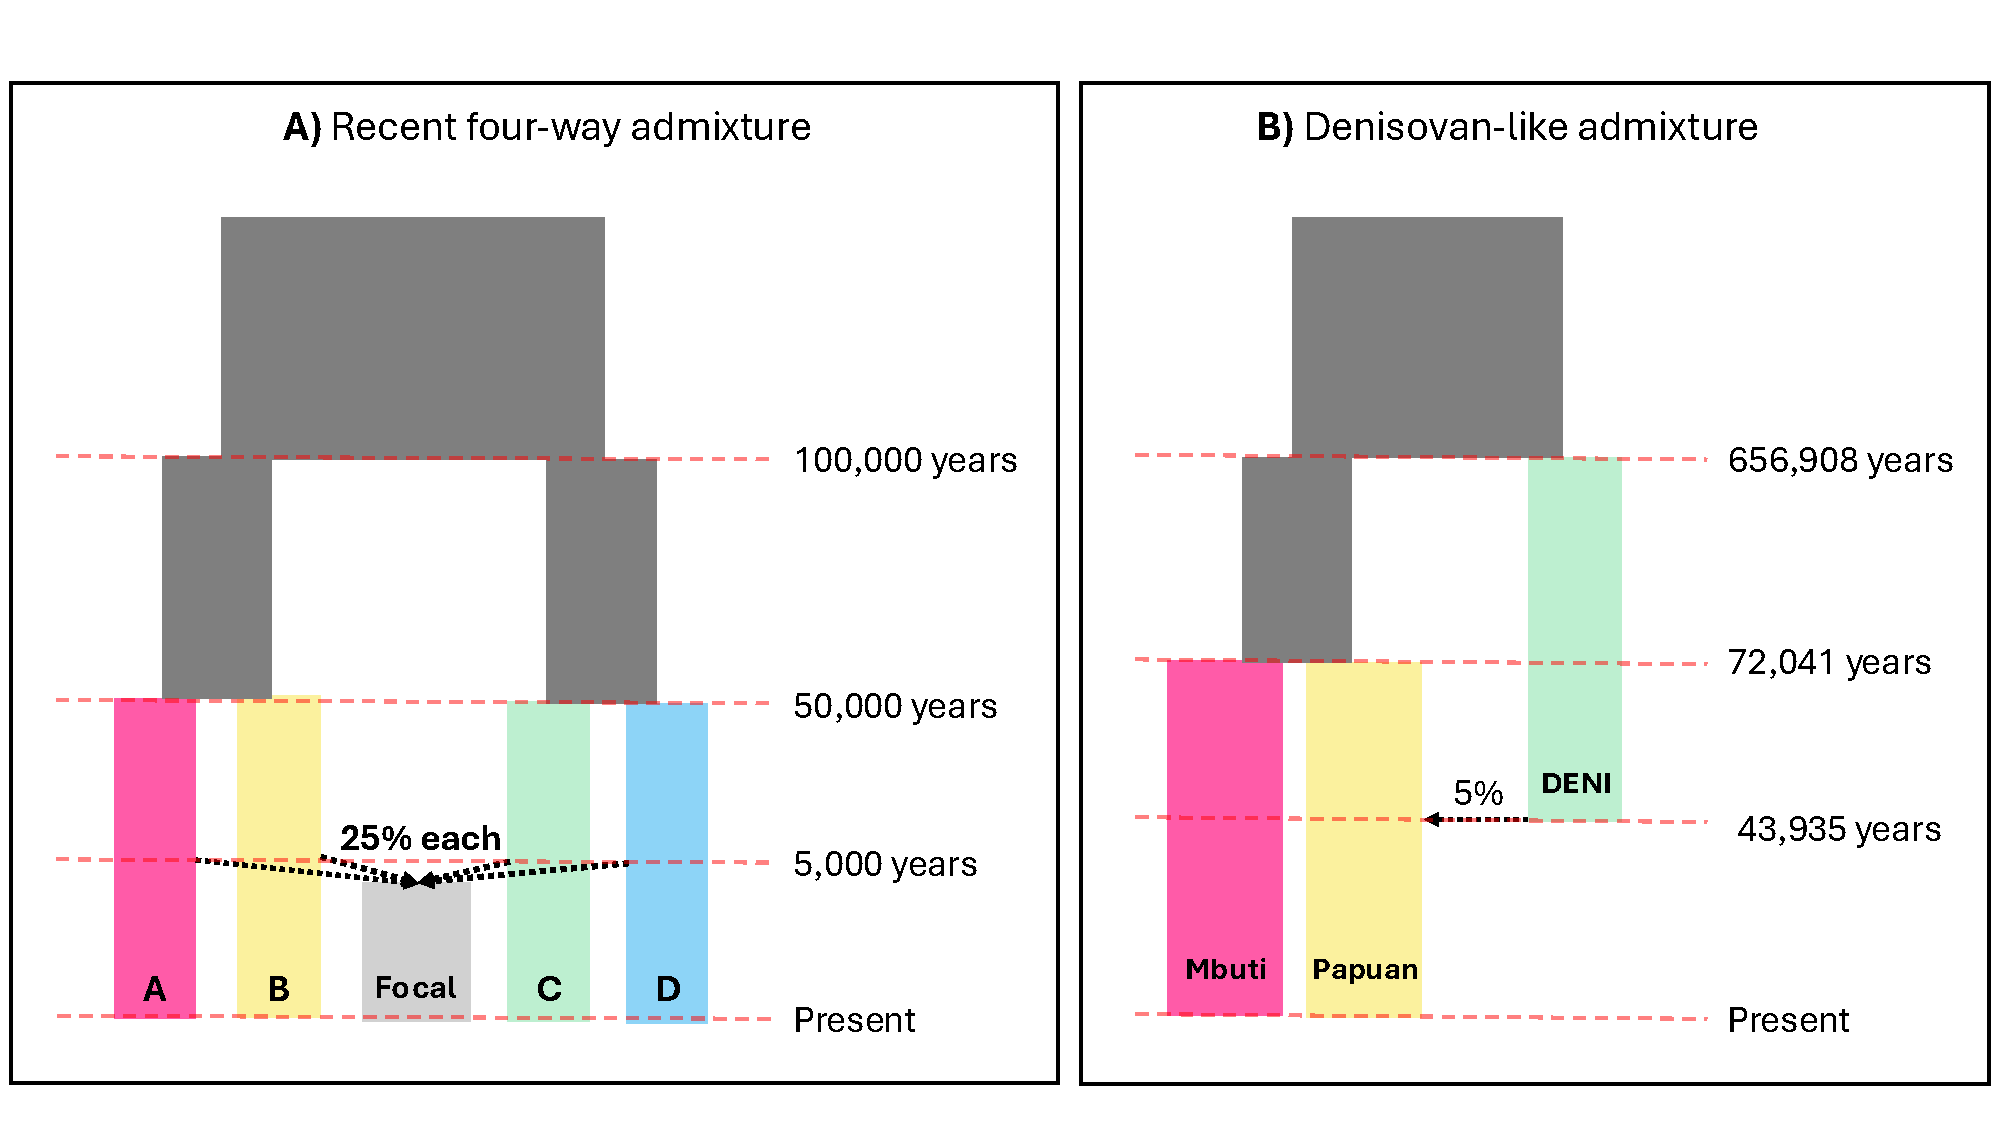
\includegraphics[width=\textwidth]{figures/thesis_gb_sim_design.pdf}
    \caption{\textbf{Simulation design for performance evaluation.} A. Four-way recent admixture simulation, B. Simulated Neanderthal introgression into Han Chinese. The simulation parameters including the population size, mutation rate and recombination map are described in section \ref{sec:ch2-gb-sim-design}.}
    \label{fig:sim1}
\end{figure}

\subsection{Four-way recent admixture}

%% para 1
% How many individuals we simulate, whats the target, whats the reference? 
% number of chromosomes? 
% We expect a 4-way admixture (see simulation design section)
% We run the method on both true trees and relate trees inferred using the variation data

We validated GhostBuster's ability to detect admixture events through a simple simulation, where we modeled a recent 4-way admixture event occurring 5,000 years ago, involving groups that had been separated for at least 50,000 years (see Figure \ref{fig:sim1}a). The focal individual in our simulation resulted from an equal contribution of 25\% ancestry from four distinct reference populations, labeled A, B, C, and D. We sampled up to 10 individuals from each reference population and used chromosomes 1 through 5. More details about the simulation setup can be found in Section \ref{sec:ch2-gb-sim-design}. Our objective was to decompose the focal individual's ancestry both with and without access to all reference populations, with the expectation of accurately identifying the four ancestral components. We applied our method primarily to trees inferred using genetic variation data via Relate, assuming a constant mutation rate of $1.25 \times 10^{-8}$, while results comparing with true trees simulated using msprime are also presented. Additionally, we only focused on coalescence events occurring from 0 to 50,000 years.

%% para 2
% We first tested the method with k=4 and presence of all reference groups
% We started with random init. and EM for 200 iterarions
% We found the four-components coal. rates represented four-populations (1 - a, 2 -b, ..)
% The coal. rates are more distinct and seperated for true trees than relate trees, representing the error in building genealogies 
% In order to compute the accuracy, we compared local ancestry with the true local ancestry R2 = 
% Calibration plots

We first tested the method with access to all four reference populations. We applied our approach to decompose the focal individual's ancestry into four components or clusters. Starting with a random initialization of coalescence rates and proportions, we fit our model over 200 EM iterations until the log-likelihood converged. The converged inverse coalescence rates represent the four clusters that maximally distinguished the coalescence events for the focal individual (see Figure xx). The inverse coalescence rate (ICR) for each component can be interpreted as the component's affinity toward one of the four reference populations—a lower ICR value indicates quicker coalescence with that specific reference population. Our analysis revealed that the four clusters identified by GhostBuster contributed roughly 25\% to the focal individual's ancestry, with each cluster closer to one of the four reference populations. For instance, component 1 was closest to population A, component 2 to population C, component 3 to population B, and component 4 to population D. When applied to true simulated trees (see Figure app1), the coalescence rates were more distinct and better separated, highlighting the fuzziness in building genealogies from genetic variation data. To assess the accuracy of our decomposition, we compared the local ancestry inferred by our EM algorithm with the simulated ground truth local ancestry. We observed a strong correlation between the local ancestry posterior inferred by GhostBuster and the ground truth, with an $R^2$ of $0.99$. Finally, we evaluated the calibration of our local ancestry estimates and found them to be well-calibrated, with an expected calibration error (ECE) of $121$ (see Figure yy).

%% para 3
% Next we removed population D from reference
% We did similar procedure with k = 4 
% four components, with the fourth component being distant from all 3 sampled reference populations
% local ancestry R2
% calibration plots

Next, we removed population D (without loss of generality) from the genealogies and attempted to decompose the focal individual. This scenario simulates the presence of a ghost population, as population D contributed to the focal individual's genetic makeup but is not included in the reference panel. We reran our method, fixing the number of components to four. The four components still contributed roughly 25\% to the total ancestry. The inverse coalescence rates (ICRs) for each component only existed for populations A, B, and C, as no individuals from population D were sampled. Component 1's ICR was closest to population A, component 2 was closest to population B, and component 3 was closest to population C (see Figure xx). However, component 4 was more distantly related to all three populations, indicating slower coalescence with each. This could be the ancestry relating to population D which could have been tagged by its slower coalescence rates with populations A-C (see Figure xx). To verify this, we compared the local ancestry inferred by running our EM algorithm without the access to population D with the simulated ground truth. We found a strong correlation, with an $R^2$ value of 0.98, indicating that component 4 effectively captured the ancestry related to population D without requiring direct samples from that population. A visual comparison of the local ancestry inferred using Relate trees, both with and without the inclusion of reference population D, is shown in Figure zz. Finally, we assessed the calibration of our local ancestry estimates in this setting and found them to be well-calibrated, with an expected calibration error (ECE) of 121 (see Figure yy).

%% para 4
% How do we choose number of components? 
% held-out validation 

We performed leave-one-chromosome-out cross-validation to determine the optimal number of components, as described in Section \ref{sec:ch2-gb-selecting-clusters}. We found that four components provided the best fit in both scenarios, whether population D was present or absent (see Figure xx).

\subsection{Denisovan-like Introgression into Papuans}

%% explain the simulation
%% with denisovan
%% without denisovan
%% comparison with skov 
%% add ablations on hmm vs no hmm, 

We examined the archaic introgression of Denisovan ancestry in modern-day Papuans by simulating an admixture event that occurred approximately 44,000 years ago, with an admixture proportion of 5\% (see Figure \ref{fig:sim1}b). The simulation parameters are from \cite{skov2018detecting}, and further details can be found in section \ref{sec:ch2-gb-sim-design}. For our analysis, we simulated 25 Papuan individuals, 25 Mbuti individuals (representing African ancestry), and a Denisovan ancient sample. We focused on chromosomes 1 through 5 for our analysis. Our objective was to decompose the Papuan individuals' ancestry both with and without access to the Denisovan sample, aiming to accurately identify Denisovan segments and admixture within Papuans. Similar to our previous simulation of a four-way recent admixture, we primarily applied our method to trees inferred from genetic variation data via Relate, assuming a constant mutation rate of $1.25 \times 10^{-8}$. Finally, we only focused on coalescence events occurring from 10,000 to 1,000,000 years for this analysis.

We begin our analysis by assuming we have access to one ancient Denisovan sample. We decompose five out of the 25 Papuan individuals, assuming two distinct components. As with the previous simulation, we randomly initialize the parameters and fit the EM algorithm for 200 iterations until the log-likelihood converges. The converged components reveal a major component, contributing around 95\% to the local ancestry, and a minor component contributing 5\% (see Figure xx). The inverse coalescence rates (ICRs) characterizing these components differ significantly. Component 1 demonstrates a slower coalescence rate with the ancient Denisovan sample and a relatively faster coalescence with the modern Mbuti samples. In contrast, component 2 exhibits a very fast coalescence with Denisovans but slower coalescence with modern Mbuti and Papuan samples. It is important to note that the most striking difference between the two components is the vastly accelerated coalescence with Denisovans in the minority group—up to over $1{,}000 \times$ faster compared to the majority group. However, there is also a substantial difference in coalescence with modern groups, which we will leverage to decompose the ancestry without access to the ancient Denisovan sample.

\begin{figure}[h!]
    \centering
    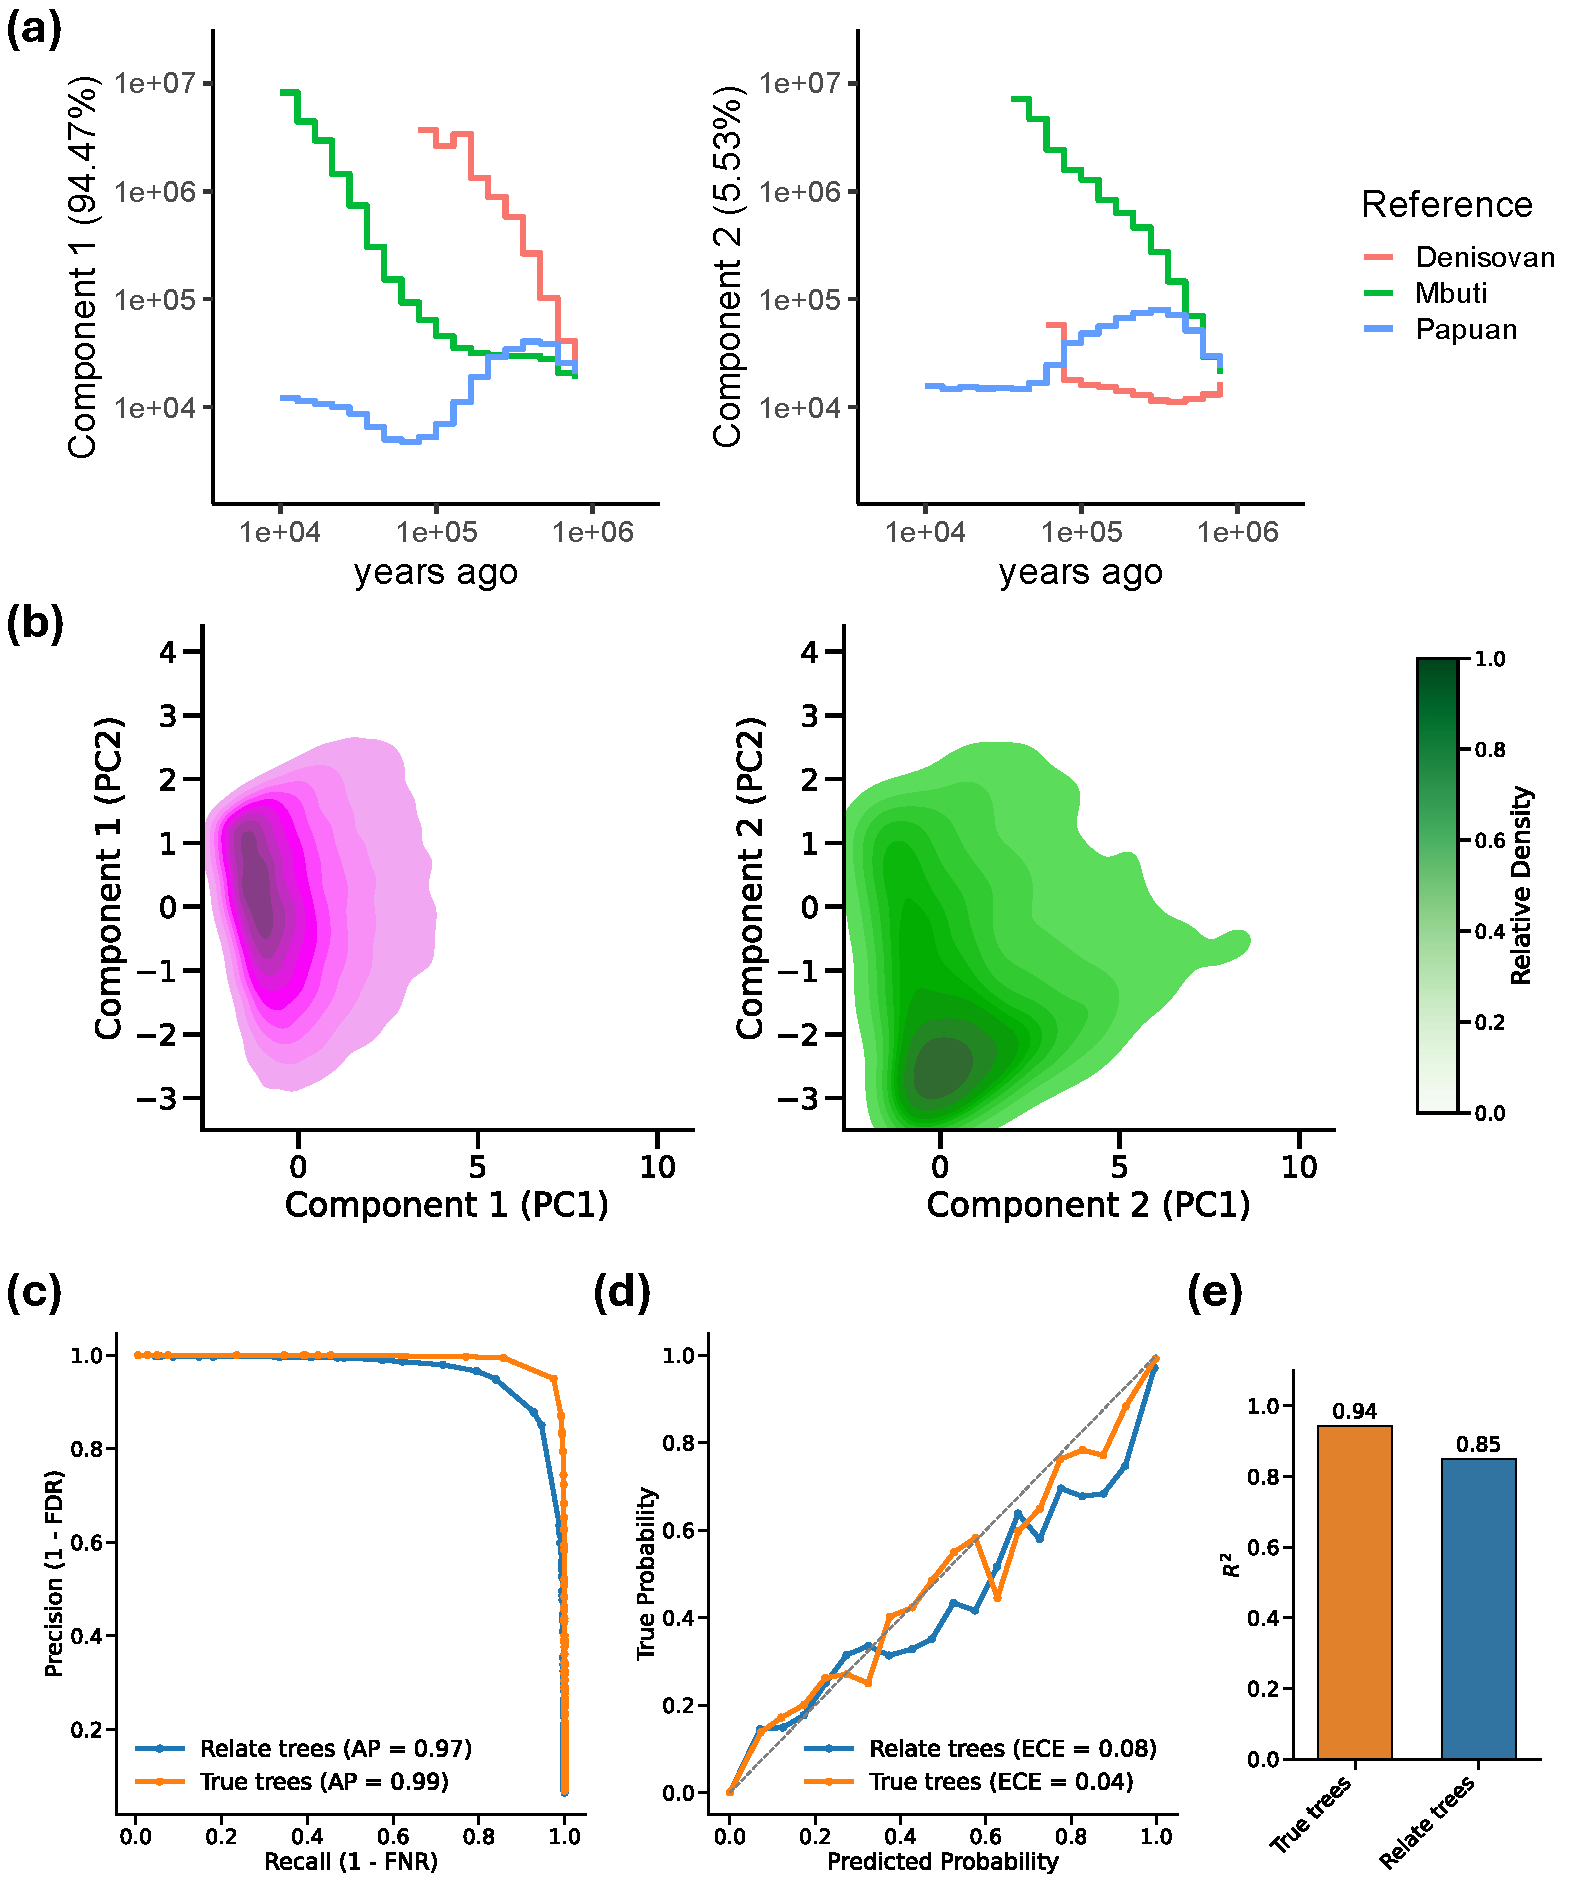
\includegraphics[width=\linewidth]{figures/gb_sims/thesis_gb_sim_denisovan_relate_ghost.pdf}
    \caption{
    \textbf{Decomposing Papuan individuals in simulations with Mbuti and Denisovans as additional references.} (a) Inferred inverse coalescence rates and proportions: each line represents inverse coalescence rate profiles with a reference population. (b) PCA visualization of the coalescence count and opportunity matrix derived from the genealogies plotted separately for each component. (c) Precision-recall curves, (d) Calibration curves, and (e) Prediction $R^2$ for inferred local ancestry compared to the simulated ground truth, where inference was done using true trees or Relate trees. The PCA visualization in (b) is based on a KDE plot with a threshold of 0.05, and binary local ancestry estimates are obtained by thresholding the inferred posteriors at 0.5.
    }
    \label{fig:enter-label}
\end{figure}

Next, we removed the Denisovan samples from our analysis and decomposed the same Papuan individuals into two components. In this scenario, the Denisovan ancestry in Papuans can be thought of as ghost population. Our method converged on two components, contributing approximately 95\% and 5\% to the local ancestry, respectively (see Figure xx). The ICRs of the minor component closely matched those of the minor component from the earlier analysis that included the Denisovan sample, showing slower coalescence with Mbuti and Papuans. Similarly, the major component demonstrated relatively faster coalescence with Mbuti and other Papuans. To verify that the minor component indeed represents Denisovan ancestry, we compared the local ancestry inferred using GhostBuster with the simulated ground-truth local ancestry. Additionally, we compared local ancestry inferences between true trees and Relate trees, both with and without access to the Denisovan sample. Our method outperformed a recent HMM-based approach tailored for detecting archaic introgression in non-Africans, yielding a higher $R^2$ value. Finally, we assessed the calibration of our local ancestry estimates and found them to be well-calibrated as shown in Figure zz.

We performed leave-one-chromosome-out cross-validation to determine the optimal number of components, as described in Section \ref{sec:ch2-gb-selecting-clusters}. We found that two components provided the best fit in both scenarios, whether Denisovan was present or absent (see Figure xx). Additionally, to test the robustness of our method, we also attempted to decompose Mbuti individuals in the same simulation, which are panmictic with no simulated population structure or admixture. We found that the likelihood corresponding to a single component outperformed the others, suggesting no admixture or significant coalescence differences among clusters.

\section{Identifying several recent admixtures accurately}
\label{sec:ch2-gb-real}

Haplotype-based methods like Alder \cite{loh2013inferring}, Globetrotter \cite{hellenthal2014genetic}, and Mosaic \cite{salter2019fine} have been instrumental in confidently inferring recent admixture events, particularly those occurring less than 1,500 years ago. We focus on several well-documented, recently admixed populations from the Human Genome Diversity Project (HGDP), including the Hazara, Bedouin, Maya, and Sindhi. Each of these populations has undergone 2- or 3-way admixture events within the past few thousand years, which have been reliably detected by previous methods. Our objective is to decompose the ancestry of individuals from these populations using GhostBuster and to compare the local ancestry with results from other haplotype-based methods.

We begin by decomposing the ancestry of Hazara individuals from the HGDP, who have been shown in previous studies to result from recent admixture between groups similar to modern-day Pathans and Mongols \cite{hellenthal2014genetic,salter2019fine}. Using all populations in our HGDP+1,000GPA dataset (as described in section \ref{sec:ch2-gb-data}), we fit two components to decompose the genome-wide ancestry of the 21 Hazara individuals. We focused on coalescence events within the last 50,000 years, dividing the time scale into 20 logarithmically spaced epochs ranging from 500 to 50,000 years. Our analysis revealed that the Hazara individuals could be decomposed into two components, each contributing roughly 50\% to the overall ancestry. The inverse coalescence rates (ICRs) indicate that component 1 is closely related to East Asian groups such as Mongols and others, while component 2 is more closely aligned with South Asian groups like the Pathans—consistent with previous findings using ChromoPainter (see Figure yy). To further validate our results, we compared the local ancestry estimates from our method with those obtained using Mosaic, which was run using all reference populations in HGDP. We found that the local ancestry was highly correlated between the two methods, with an $R^2$ of 0.92. Potential differences in local ancestry estimates may be attributed to additional steps in Mosaic, such as correction for phasing, which are not present in our method. Additionally, when we excluded South Asian samples from the reference panel, we still identified similar components with comparable local ancestry inference, though the correlation with Mosaic decreased ($R^2 = 0.61$, see Figure xx). 

We conducted similar analyses for other populations in the HGDP, including the Bedouin (with European and African admixture), Maya (with African, Native American, and European admixture), and the Sindhi and Druze populations (both of which exhibit East Asian and South Asian admixture). The proportions of admixture, potential source populations, and estimated timing of these admixture events for each population are summarized in Table xx. A more detailed analysis for each population, along with visual representations, can be found in the appendix (see Figures xx, yy, zz, and aa).